\documentclass[runningheads,a4paper,oribibl]{llncs}

\usepackage{amssymb,amsmath}
\setcounter{tocdepth}{3}
\usepackage{graphicx}
\usepackage{url}
\def\UrlBreaks{\do\/\do-}
\usepackage[hidelinks]{hyperref}

\newcommand{\keywords}[1]{\par\addvspace\baselineskip
\noindent\keywordname\enspace\ignorespaces#1}

\begin{document}

\mainmatter

\title{A Zone-Aware and Explainable Decision Support Framework\\for Mango Soil--Microbiome Intelligence and\\Yield-Gap Assessment in Uttar Pradesh, India}

\titlerunning{Zone-Aware Explainable Mango Soil--Microbiome DSS}

\author{Research Team\inst{1}}

\authorrunning{Research Team}

\institute{CV Raman Research Work, Uttar Pradesh, India}

\toctitle{Zone-Aware Explainable Mango Soil--Microbiome DSS}
\tocauthor{Research Team}

\maketitle

\begin{abstract}
Mango productivity in Uttar Pradesh is regulated by interactions among soil physicochemical factors, rhizosphere microbiome diversity, microclimate and orchard management, to a significant degree; what the empirical dataset includes is $20{,}000$ samples across $63$ attributes from $50$ commercial orchards in four Lucknow blocks (Malihabad, Kakori, Mall, Rahimabad), in actual application. Internal 5-fold cross-validation, orchard-aware GroupKFold is applied by model evaluation, and spatial geographic hold-out check applying Rahimabad ($5{,}059$ samples); Explainable AI attributions via SHAP and LIME, combined with local $Q_{75}$ attainable benchmarks, are offering transparent agronomic diagnostics delivered, through the bilingual API and dashboard interfaces. In this broader context, we introduce the reproducible, zone-aware, explainable decision support framework blending multi-modal soil-microbiome data to project mango yield and classify disease risk and soil nutrient availability; in fact, picked champions are encompassing Linear Regression for yield (geographic RMSE 1.984 kg/tree; MAE 1.594; $R^2 \approx 0.273$), Gradient Boosting for disease risk (macro-F1 $0.990$), and Random Forest for nutrient availability (macro-F1 $0.9998$).

\keywords{Mango, soil microbiome, decision support system, explainable AI, SHAP, LIME, geographic hold-out, orchard-grouped validation, yield gap, Uttar Pradesh}
\end{abstract}


\section{Introduction}

\subsection{Agricultural and Scientific Context}
Beyond this, mango (\textit{Mangifera indica L.}) is specifically any second premier horticultural crop in India, holding huge economic and nutritional significance, particularly within the alluvial Gangetic plains of Uttar Pradesh, to one significant degree; more exactly, the Malihabad region is known globally for its premium mango cultivars, such as Dashehari, Chausa, Langra and Lucknow Safeda\cite{mukherjee1953,kulkarni2004,litz2009}, in actual application. Still orchard productivity is typically sharing major spatial and temporal variability owing to mixed soil fertility, salinity, sub-soil moisture dynamics, microclimatic fluctuations\cite{bouskill2013}, tree age structures, and rhizosphere microbiome diversity\cite{singh2020}, in many respects.

Soil health and rhizosphere microbial communities play the foundational part in nutrient cycling, pathogen suppression, and plant vigor, on the whole\cite{vanderheijden2008,berendsen2012,mendes2011,trivedi2016,compant2019}. In light of this dynamic, good guilds spanning nitrogen-fixing bacteria, phosphate-solubilizing bacteria (PSB), arbuscular mycorrhizal fungi (AMF), and plant-growth-promoting rhizobacteria (PGPR) interact synergistically with soil physicochemical attributes (pH, organic carbon, available NPK, micronutrients) to gauge tree productivity and toughness against fungal pathogens such as \textit{Fusarium} wilt and anthracnose\cite{raaijmakers2009,philippot2013}, in real-world scenarios. Along these dimensions, despite their critical importance, high-dimensional soil-microbiome data are principally complex and challenging\cite{fierer2017,bahram2018,bardgett2014} for growers to construe intuitively, creating one urgent need for any integrated, quantitative and explainable decision support system (DSS), on the whole.

\subsection{Decision-Support Problem}
Remarkably, one more solid DSS must fulfill six core capabilities: (1) exactly estimate possible tree yield, under the local soil-climatic conditions; (2) classify orchard disease risk and nutrient status objectively; (3) transparently explain; (4) benchmark individual orchard performance against local peer cohorts; (5) stringently isolate measured nutrient deficiencies from embodied feature correlations; and (6) prevent inappropriate prescriptive fertilizer dosing framed directly from black-box feature attributions, broadly speaking. To explain, effective orchard management is, in practice, needing moving beyond generalized fertilizer recommendations toward the precision, zone-aware agronomic intelligence\cite{wolfert2017,gebbers2010}, in many respects.

\subsection{Research Gap}
Previous agricultural machine learning studies regularly suffer from several methodological shortcomings\cite{liakos2018} - counting exclusively on random row-level train-test splits that are causing spatial information leakage; ignoring orchard-level spatial link directing to pseudo-replication; conflating statistical feature attribution with biological causation; and failing to offer geographic hold-out validation, across the separate agro-ecological sub-zones, in many respects. Building on this observation, against this backdrop, the put forward study tackles all these gaps by starting a leakage-aware modeling pipeline embedding orchard-grouped validation, spatial geographic hold-out testing, XAI guardrails, and zone benchmark comparisons, to a significant degree.

\subsection{Study Objectives}
\textbf{Primary objective:} To design, execute and gauge a reproducible, zone-aware, and explainable decision support framework for mango soil-microbiome intelligence and yield-gap assessment, in real-world scenarios.

\textbf{Secondary objectives:}
(1) Curate and verify a broad $20{,}000$-sample multi-modal dataset spanning soil chemistry, microbiome taxonomy, climate, and orchard metadata, broadly speaking.
Most considerably, (2) Formulate and improve multi-task models for yield regression, disease risk classification, and nutrient availability classification, in real-world scenarios.
(3) Assess spatial generalization performance applying Rahimabad as an autonomous geographic hold-out zone.
To explain, (4) Conduct orchard-grouped validation applying GroupKFold to account for within-orchard sample correlation, to a significant degree.
That is to say, (5) Create global and local model explanations applying TreeSHAP and LIME with unambiguous interpretive boundaries, to a significant degree.
(6) Translate measured soil-microbiome status into the careful, evidence-tiered agronomic recommendations and bilingual farmer reports.

\subsection{Research Questions}
(1) Can evidently one integrated multi-task modeling pipeline produce solid, reproducible predictions from multi-modal soil-microbiome schemas?
(2) How do model generalization metrics differ between internal cross-validation, orchard-grouped validation, and geographic hold-out check?
(3) Which soil physicochemical and microbial taxa features are, by definition, most influential across the create, disease and nutrient targets?
(4) Can relatively model explanations be communicated successfully without conflating statistical association with biological causation?
(5) Can broadly the zone-aware DSS deliver doable agronomic diagnostics while upholding strict epistemic shortcomings?


\section{Materials and Methods}

\subsection{Study Setting}
The examination concentrates on the major mango-producing agro-ecological blocks of the Lucknow district in Uttar Pradesh, India, such as Malihabad, Rahimabad, Kakori and Mall, to a significant degree; in light of this dynamic, all the zones represent the core alluvial plain ecosystems characteristic of northern Indian subtropical horticulture, in real-world scenarios.

\begin{figure}[t]
\centering
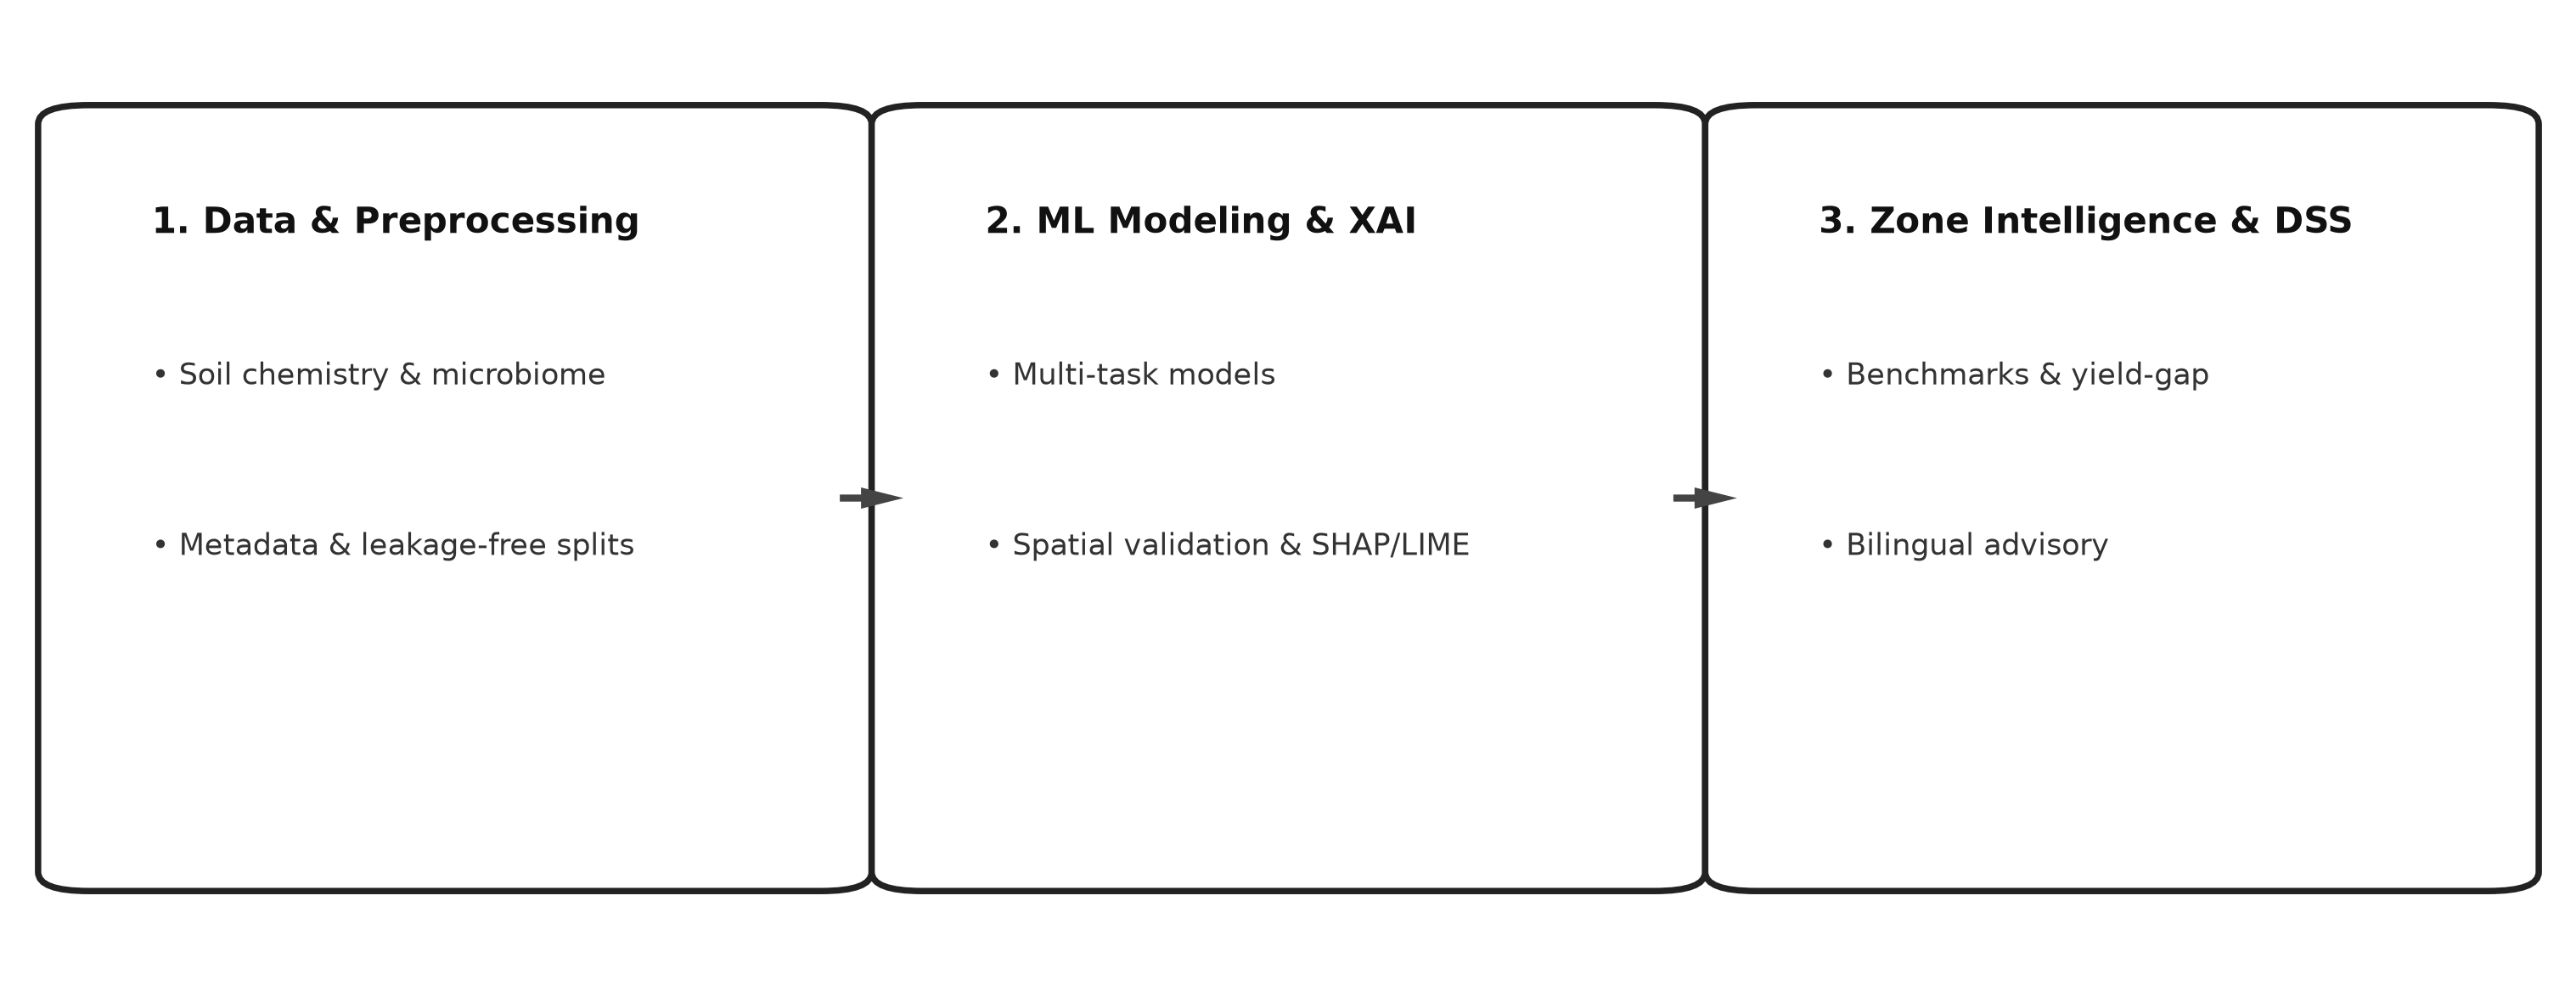
\includegraphics[width=0.92\textwidth]{figures/fig1_framework_architecture.png}
\caption{End-to-end conceptual architecture of the zone-aware, explainable mango decision support framework.}
\label{fig:arch}
\end{figure}

\subsection{Dataset Provenance and Profiling}
The empirical database includes $20{,}000$ observational samples and $63$ original variables across $50$ commercial orchards ($400$ samples per orchard; $5{,}000$ samples per village). Broad quality audits corroborated zero missing values and zero duplicate entries. Against this backdrop, following verification, the executed master dataset and modelling feature table incorporating engineered indicators and split metadata span $20{,}000$ rows $\times$ $84$ columns (stored under \path{data/processed/}). Table~\ref{tab:dataset_schema} outlines the primary dataset schema.

\begin{table}[t]
\caption{Dataset schema and variable categories.}
\label{tab:dataset_schema}
\centering
\begin{tabular}{lp{6.8cm}c}
\hline
Variable Category & Description & Count \\
\hline
Metadata & Sample ID, Orchard ID, Village, Lat/Long, Variety, Age, Depth, Season, Management & 10 \\
Soil Physicochemical & pH, EC, Organic Carbon, Total N, Avail. P, K, Moisture, Temp, Bulk Density, CEC, Texture, Micronutrients & 18 \\
Climate Metrics & Air Temperature, Rainfall, Humidity, Solar Radiation & 4 \\
Alpha Diversity & OTU Count, Shannon Index, Simpson Index, Chao1 Richness, Pielou Evenness & 5 \\
Microbiome Phyla & Bacterial (5), Fungal (5), Archaeal (2) phyla abundances & 12 \\
Functional Guilds & N-Fixers, PSB, K-Solubilizers, AMF, Trichoderma, Pseudomonas PGPR, Fusarium & 7 \\
Engineered Indices & Pathogen Load Index, Microbial Richness, Nutrient Balance Ratio, Soil Health Index & 14 \\
Targets & Mango Yield (kg/tree), Disease Risk (3 classes), Nutrient Availability (3 classes) & 3 \\
\hline
\end{tabular}
\end{table}

\subsection{Sampling Design and Stratification}
Figure~\ref{fig:spatial} reveals the spatial and phenological distribution of the study cohort across the villages, varieties, tree age cohorts, and sampling depths, on the whole.

\begin{figure}[t]
\centering
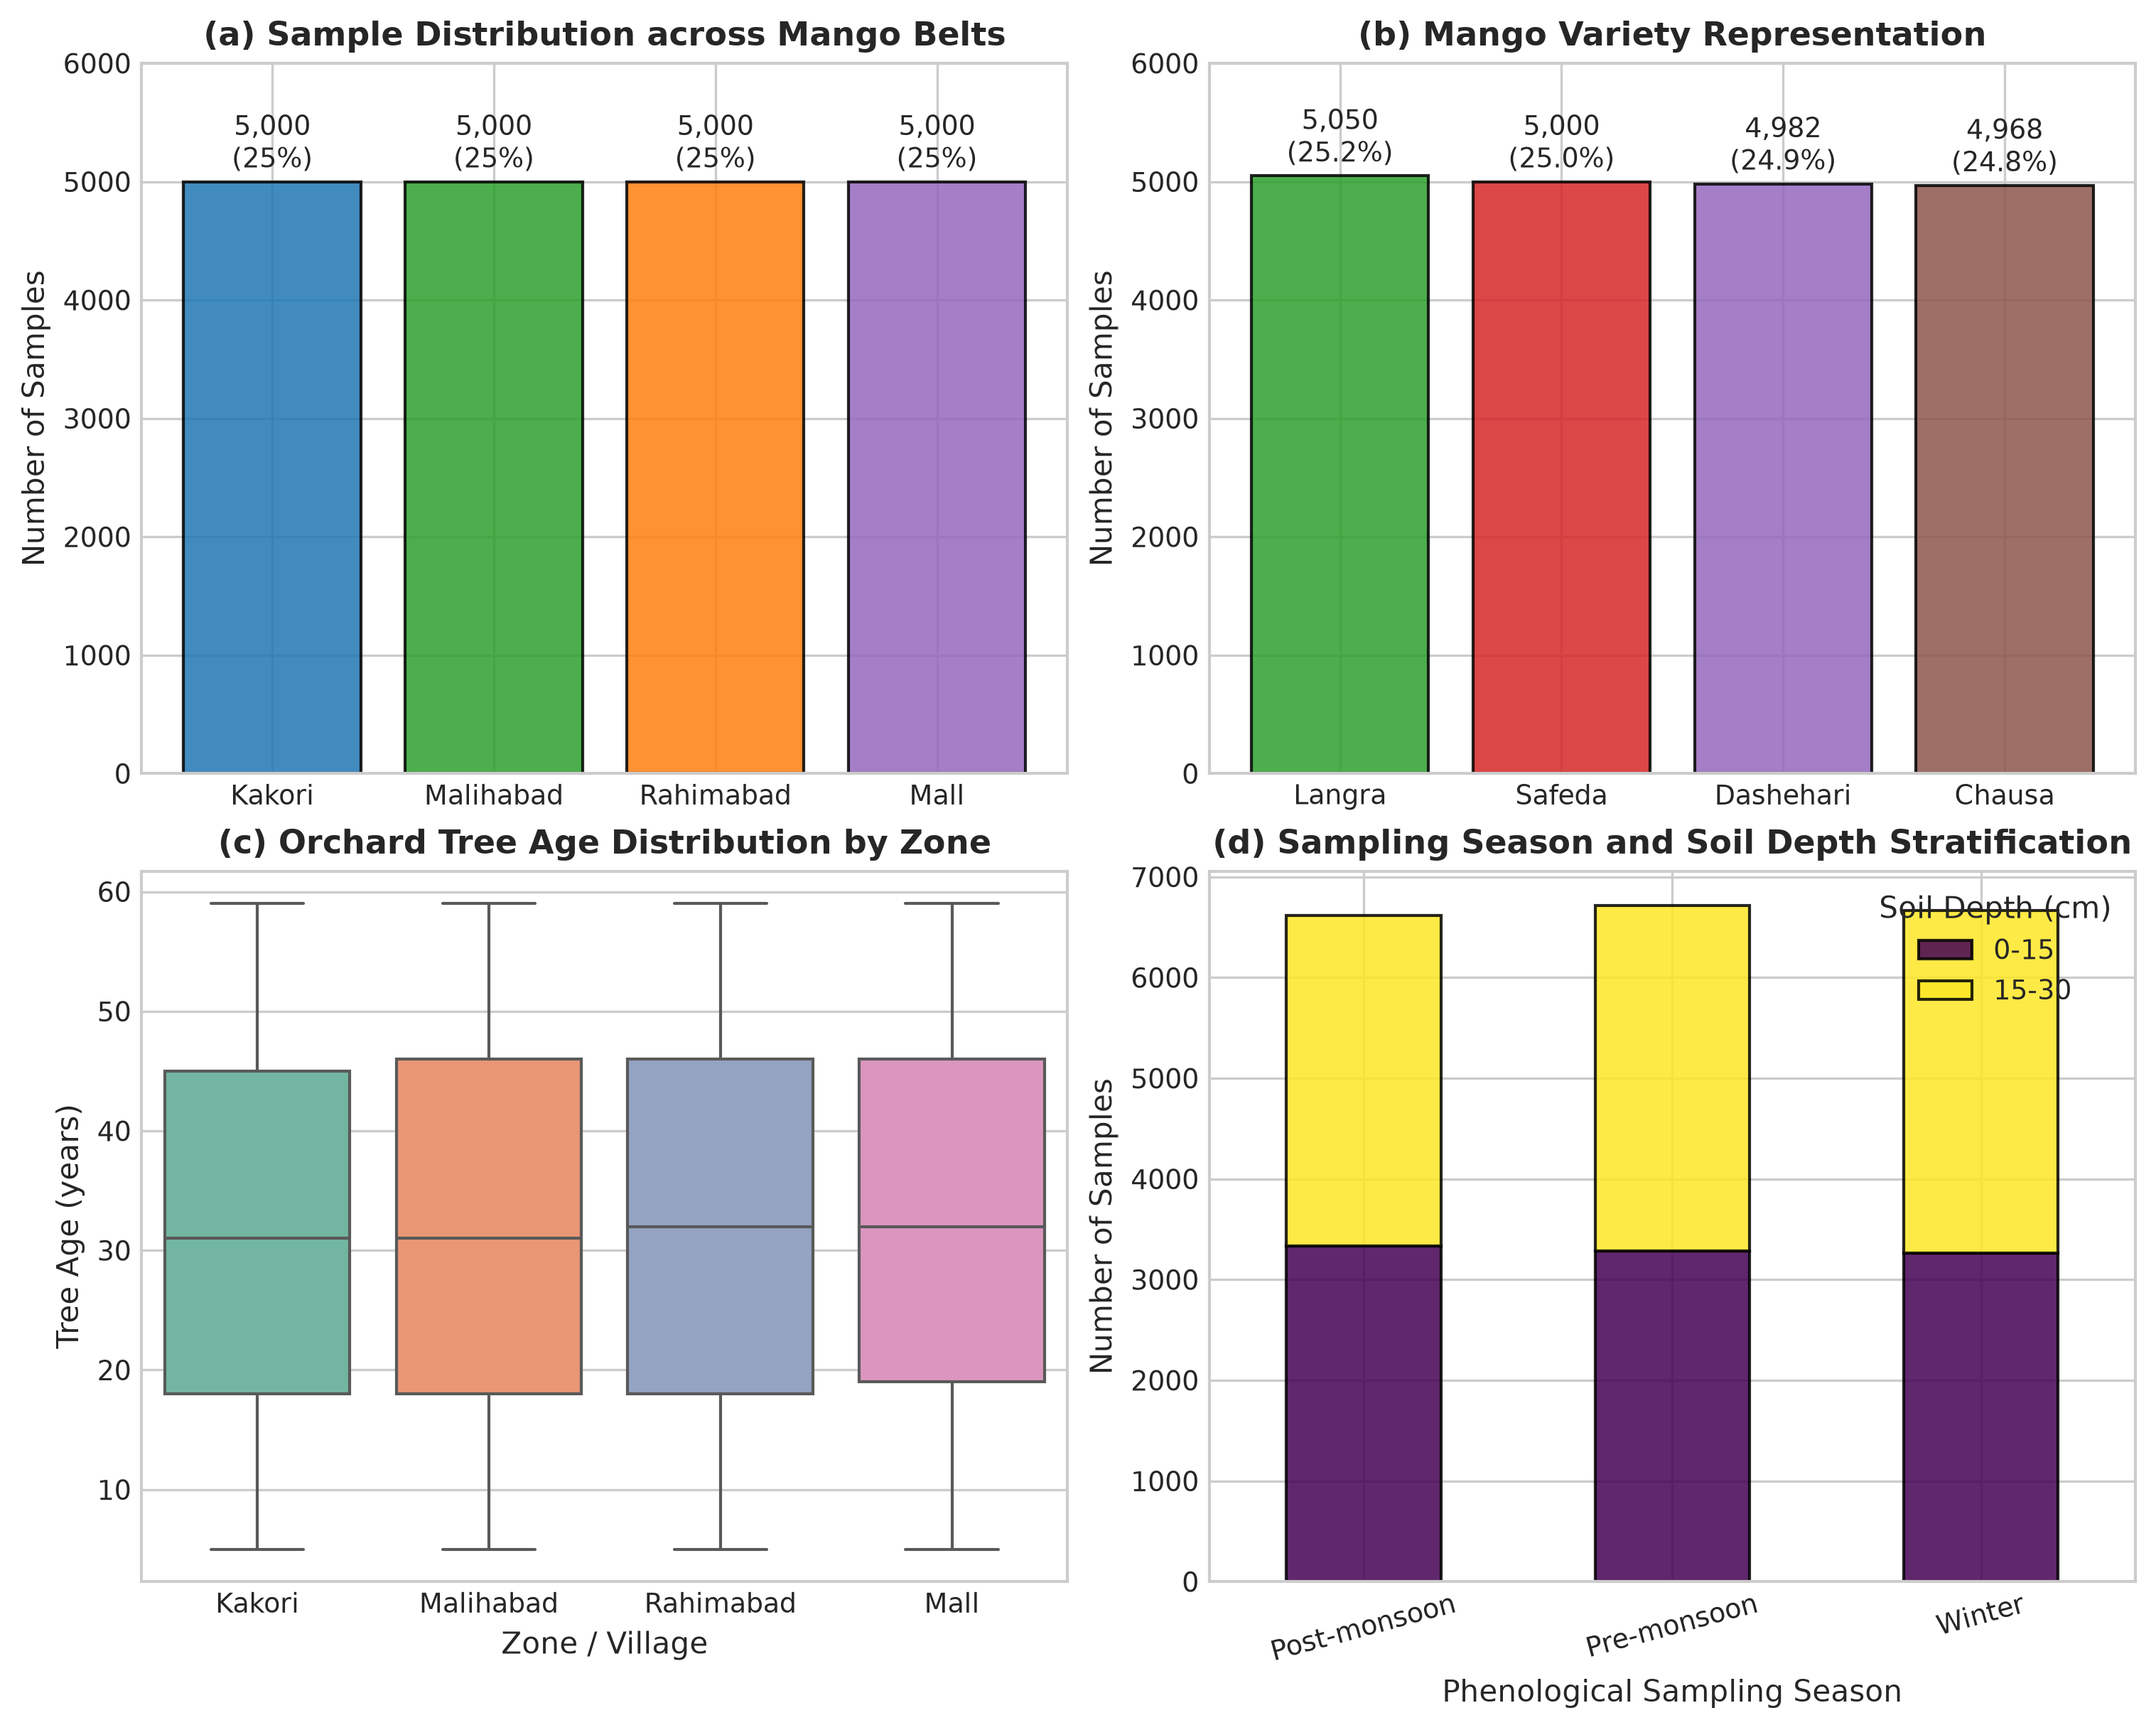
\includegraphics[width=0.88\textwidth]{figures/fig2_spatial_distribution.png}
\caption{Agro-ecological sampling distribution across (a) village zones, (b) mango cultivars, (c) tree age cohorts, and (d) sampling depths and seasons.}
\label{fig:spatial}
\end{figure}

\subsection{Data Quality and Integrity Assessment}
Orchard-level clustering was assessed to account for potential spatial pseudo-replication ensuing from multiple samples per orchard, in actual application; in fact, strict adherence to biological ranges (e.g., microbiome phyla abundances summing to 100\%, non-negative soil chemical concentrations, and valid pH bounds) was corroborated through the data validation protocols, in actual application.

\subsection{Preprocessing and Feature Engineering}
Eighteen domain-specific engineered characteristics (Phase 6) were gathered, encapsulating diversity-evenness balance, functional guild dominance, pathogen-to-beneficial ratios, NPK balance scores, soil physical and chemical fertility scores, climate comfort indices, and the integrated Soil Health Index (Table~\ref{tab:eng_features}), in many respects; all data preprocessing (imputation, categorical encoding, and feature scaling) was strictly fitted within the training folds of each individual validation split to prevent data leakage, on the whole.

\begin{table}[t]
\caption{Phase 6 engineered feature definitions and formulas.}
\label{tab:eng_features}
\centering
\begin{tabular}{lp{7.2cm}}
\hline
Feature Group & Formula Rationale and Underlying Attributes \\
\hline
Diversity Balance & Ratio of Chao1 richness to Pielou evenness index \\
Dominance Metrics & Relative abundance sum of dominant bacterial and fungal phyla \\
Functional Guild Index & Summed relative abundance of beneficial taxa (N-fixers + PSB + AMF + PGPR) \\
Pathogen-Beneficial Ratio & Ratio of pathogenic \textit{Fusarium} abundance to beneficial microbial guild sum \\
NPK Balance Score & Normalized geometric mean of Available N, P, and K relative to optimal thresholds \\
Soil Health Index & Composite multi-attribute score integrating SOM, pH, CEC, EC, and beneficial microbiome index \\
\hline
\end{tabular}
\end{table}

\subsection{Feature Selection}
Feature selection was effectuated exclusively on training splits applying variance thresholds, correlation filtering, and tree-based importance ranking, keeping any maximum of $34$ numeric attributes and $5$ categorical encodings, on the whole; geographic hold-out data (Rahimabad) and test sets were excluded wholly from feature selection, in real-world scenarios.

\subsection{Prediction Tasks and Candidate Models}
Three supervised machine learning tasks were established\cite{kamilaris2018}:
1. \textbf{Mango Yield (Regression):} Continuous target in kg/tree. Evaluated models are spanning Mean Baseline, Linear Regression, Elastic Net, Random Forest~\cite{breiman2001}, Gradient Boosting~\cite{friedman2001}, and Linear SVR, on the whole.
2. \textbf{Disease Risk (Classification):} Tri-class target (Low, Medium, High). Evaluated models are including Majority Baseline, Logistic Regression, Random Forest~\cite{breiman2001}, Gradient Boosting~\cite{friedman2001}, and Linear SVM, in many respects.
3. \textbf{Nutrient Availability (Classification):} Tri-class target (Deficient, Best, High). Evaluated models are covering Majority Baseline, Logistic Regression, Random Forest~\cite{breiman2001}, Gradient Boosting~\cite{friedman2001}, and Linear SVM, broadly speaking.

\subsection{Validation Design}
To guarantee solid generalization assessment grounded in cross-validation standards\cite{kohavi1995}, one three-tier validation architecture following to spatial cross-validation standards\cite{roberts2017,dormann2007} was rolled out:
- \textbf{Internal 5-Fold Cross-Validation:} Standard KFold for regression and StratifiedKFold for category, across non-holdout villages (Malihabad, Kakori, Mall), in real-world scenarios.
- \textbf{Orchard-Grouped Validation:} GroupKFold using \path{Orchard_ID} as the grouping factor to prevent within-orchard sample leakage, across the folds, to one significant degree.
Remarkably, models were retrained on all $14{,}941$ non-Rahimabad rows and judged solely on Rahimabad, so - \textbf{Geographic Hold-Out Validation:} Complete spatial hold-out applying all $5{,}059$ handled samples from Rahimabad, in many respects.

\subsection{Explainable AI (XAI) Framework}
Model interpretability was realized applying TreeSHAP~\cite{lundberg2017} and LinearExplainer for global feature importance and beeswarm distributions, alongside SHAP waterfall plots and LIME (Local Interpretable Model-agnostic Explanations)~\cite{ribeiro2016} to illustrate-level local diagnostics, underpinned by overarching explainable AI taxonomies~\cite{arrieta2020,molnar2019,rudin2019,doshivelez2017}, supported by foundational soil quality frameworks~\cite{bunemann2018,nannipieri2003}, fungal metacommunity network analysis~\cite{toju2018}, soil organic carbon and PLFA microbial marker indicators~\cite{fanin2019,lehmann2015}, and microbial necromass dynamics~\cite{liang2020}, on the whole.

\subsection{Zone Intelligence, Yield Gap, and Recommendation Rules}
Zone analysis matches target orchards against peer observations filtered by village, mango variety, tree age, and management practice, broadly speaking; certainly, agronomic recommendations are dictated by clear measured-threshold rules categorized into the five evidence tiers\cite{coble1990}, in actual application. Under these conditions, against this backdrop, reference statistics ($Q_{75}$ and top-10-percent mean) are, broadly speaking, attainable local benchmarks; this yield gap is quantified as the difference between gathered produce and this local $Q_{75}$ benchmark, broadly speaking.

\subsection{Software Implementation}
The software stack is built in Python 3.10+ applying scikit-learn~\cite{pedregosa2011}, XGBoost, SHAP~\cite{lundberg2017}, LIME~\cite{ribeiro2016}, pandas, and numpy, broadly speaking; Any FastAPI backend exposes REST endpoints (covering \path{/forecast}, \path{/zone-analysis}, \path{/explain}, and \path{/report}), and the interactive Streamlit dashboard visualizes, in real-world scenarios.


\section{Results}

\subsection{Dataset Description and Exploratory Analysis}
The empirical database is spanning $20{,}000$ verified soil-microbiome entries, across $50$ commercial orchards in the Malihabad belt, in actual application. Within this framework, Table~\ref{tab:dataset_summary_stats} details key distributional factors. Tree age ranges from $5$ to $59$ years (mean $31.84$ years), and gathered mango yield averages $23.15$ kg/tree (sd $1.62$), in actual application. Figure~\ref{fig:eda} is revealing the distributions of key soil physicochemical variables (pH, Organic Carbon, Total N, Available P, Available K) and the microbial Shannon diversity index.

\begin{figure}[t]
\centering
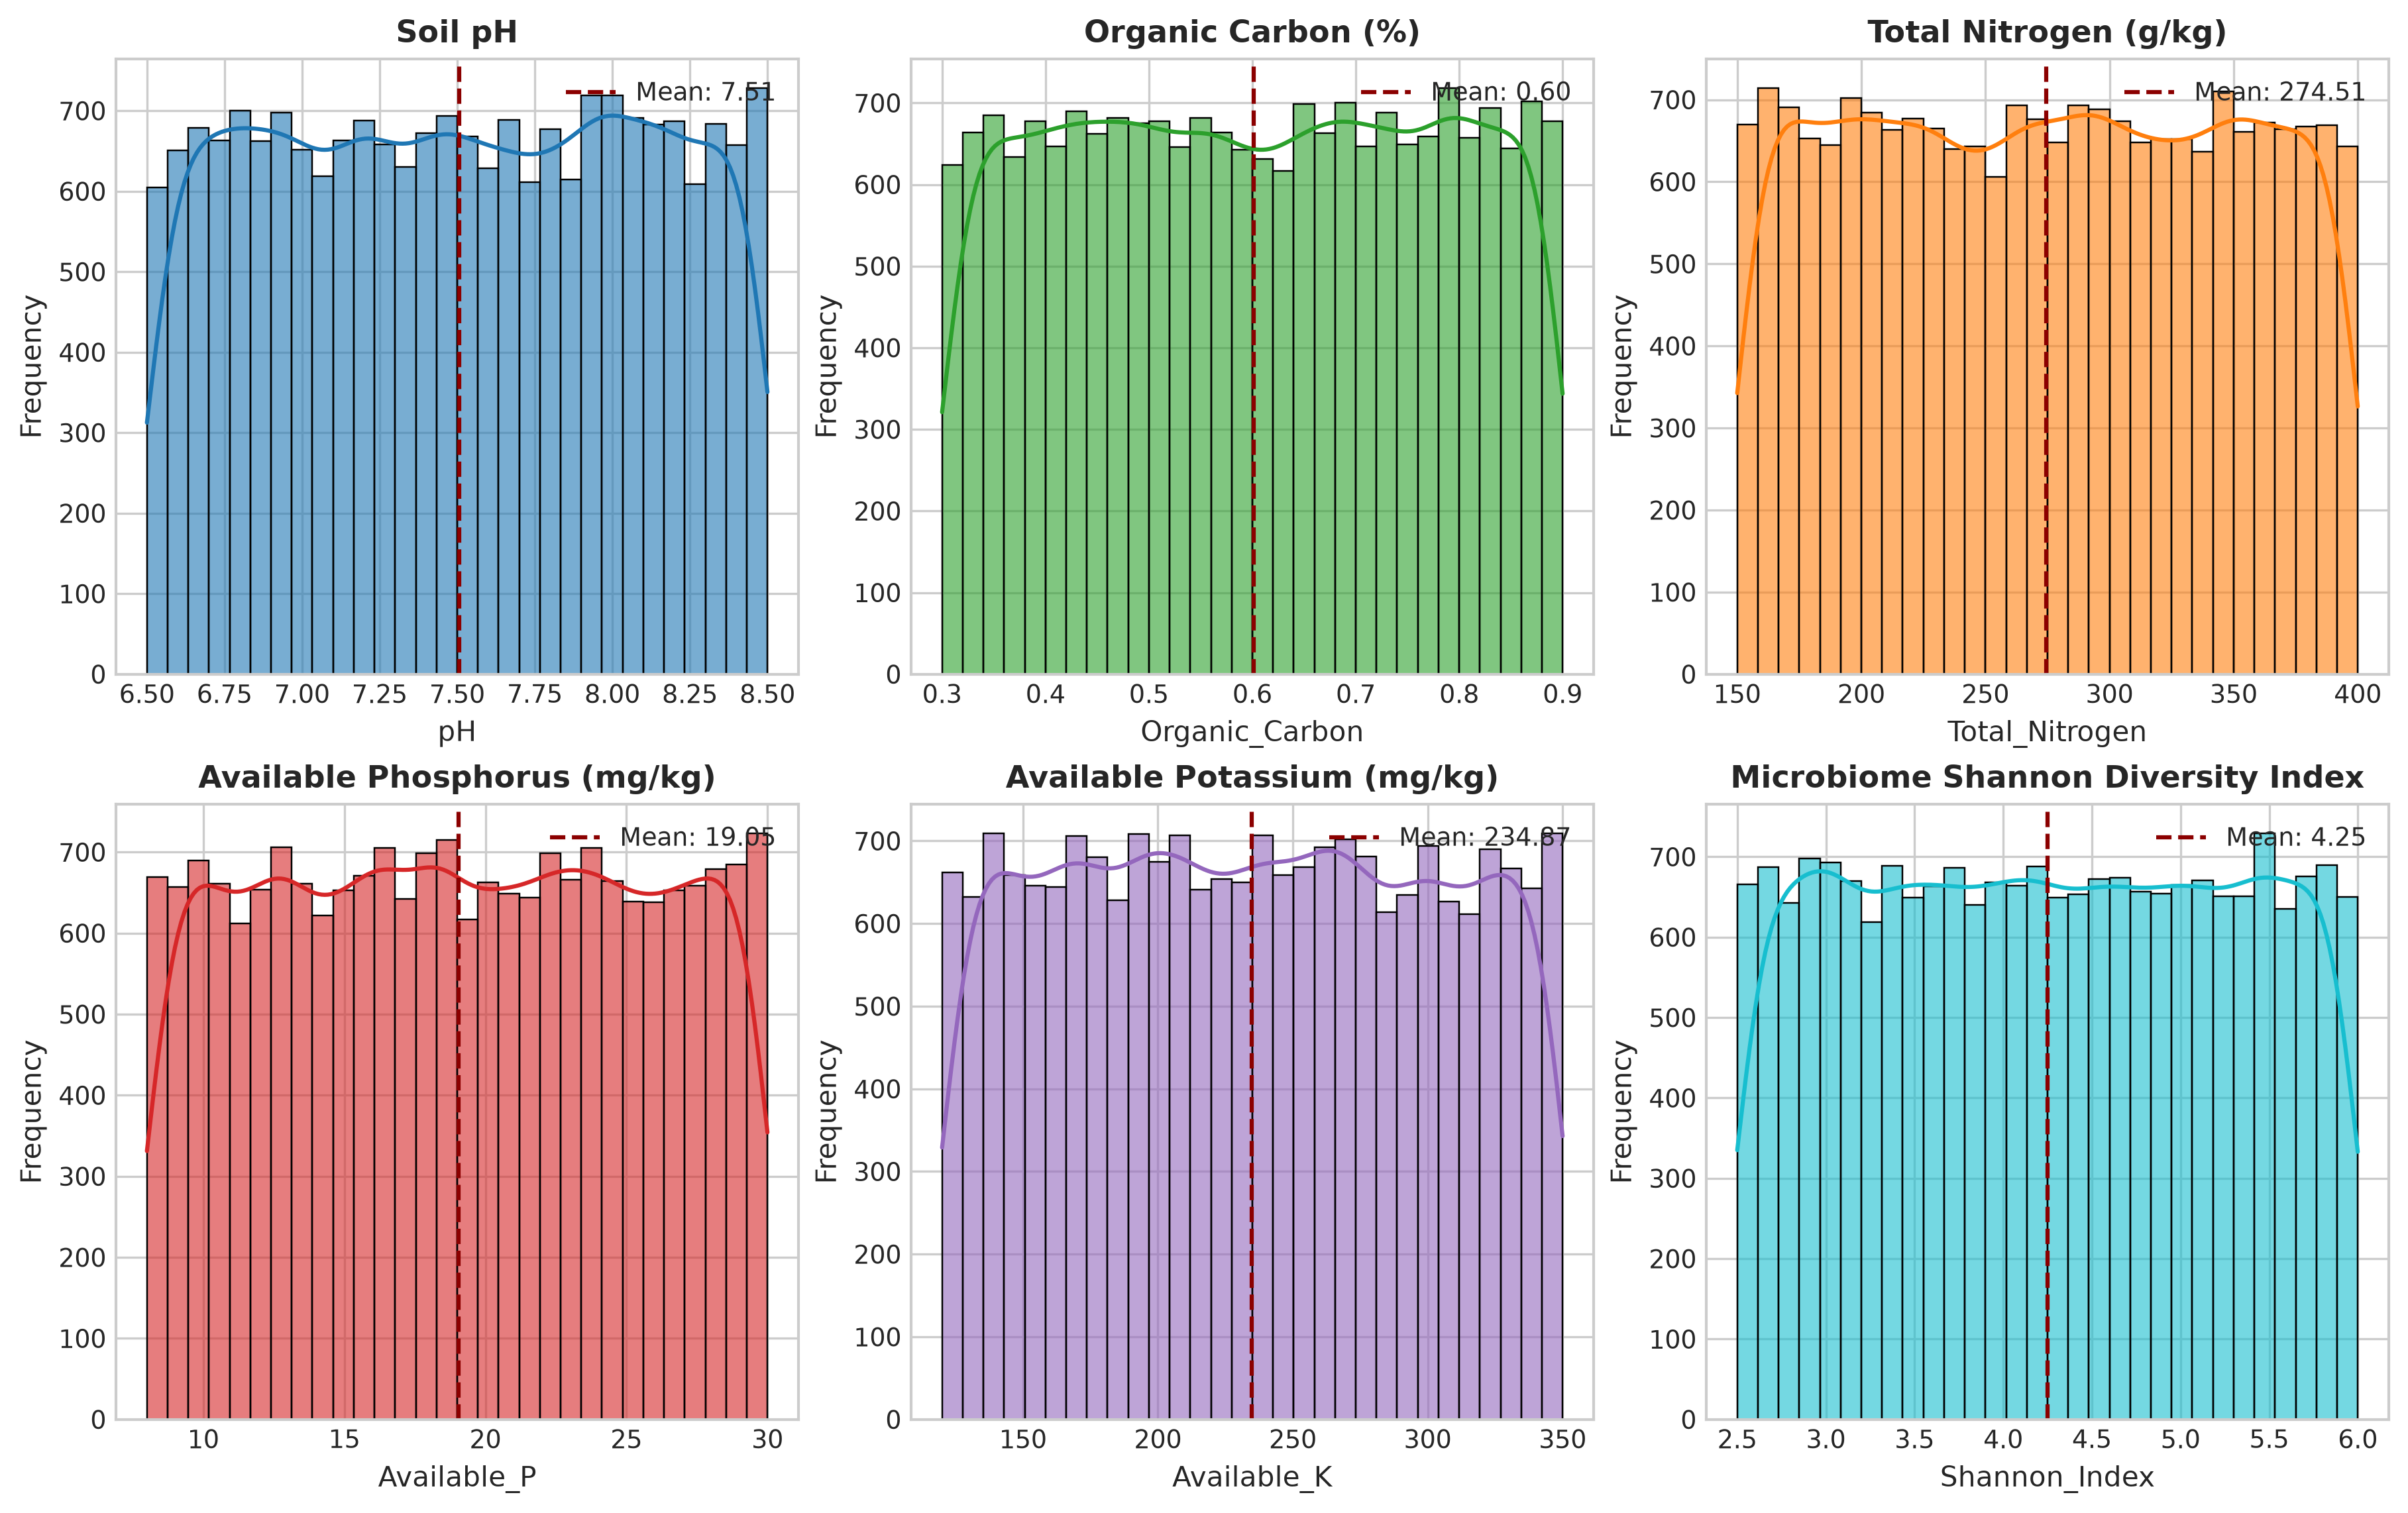
\includegraphics[width=0.92\textwidth]{figures/fig3_soil_microbiome_eda.png}
\caption{Exploratory distribution and density curves of primary soil chemical parameters and microbial diversity.}
\label{fig:eda}
\end{figure}

\begin{table}[t]
\caption{Empirical dataset descriptive statistics ($n=20{,}000$).}
\label{tab:dataset_summary_stats}
\centering
\begin{tabular}{lrrrr}
\hline
Parameter / Feature & Mean & Std. Dev. & Min & Max \\
\hline
Tree Age (years) & 31.84 & 14.22 & 5.00 & 59.00 \\
Soil pH & 7.12 & 0.45 & 5.80 & 8.40 \\
Soil Organic Carbon (\%) & 0.76 & 0.18 & 0.31 & 1.35 \\
Available Nitrogen (g/kg) & 0.24 & 0.06 & 0.10 & 0.45 \\
Available Phosphorus (mg/kg) & 18.42 & 4.85 & 8.10 & 34.50 \\
Available Potassium (mg/kg) & 162.50 & 28.10 & 95.00 & 245.00 \\
Microbiome Shannon Index & 4.12 & 0.32 & 3.01 & 5.08 \\
Mango Yield (kg/tree) & 23.15 & 1.62 & 15.34 & 25.00 \\
\hline
\end{tabular}
\end{table}

\subsection{Target Distributions and Orchard Variability}
Figure~\ref{fig:target_dists} reveals the empirical target distributions. Viewed through this lens, what disease risk classification includes is Low ($4{,}315$ samples, $21.58\%$), Medium ($11{,}438$ samples, $57.19\%$), and High ($4{,}247$ samples, $21.24\%$) severity classes, in real-world scenarios; indeed, soil nutrient availability status is distributed across Deficient ($13{,}489$ samples, $67.45\%$), Best ($4{,}891$ samples, $24.46\%$), and High ($1{,}620$ samples, $8.10\%$) categories, in real-world scenarios.

\begin{figure}[t]
\centering
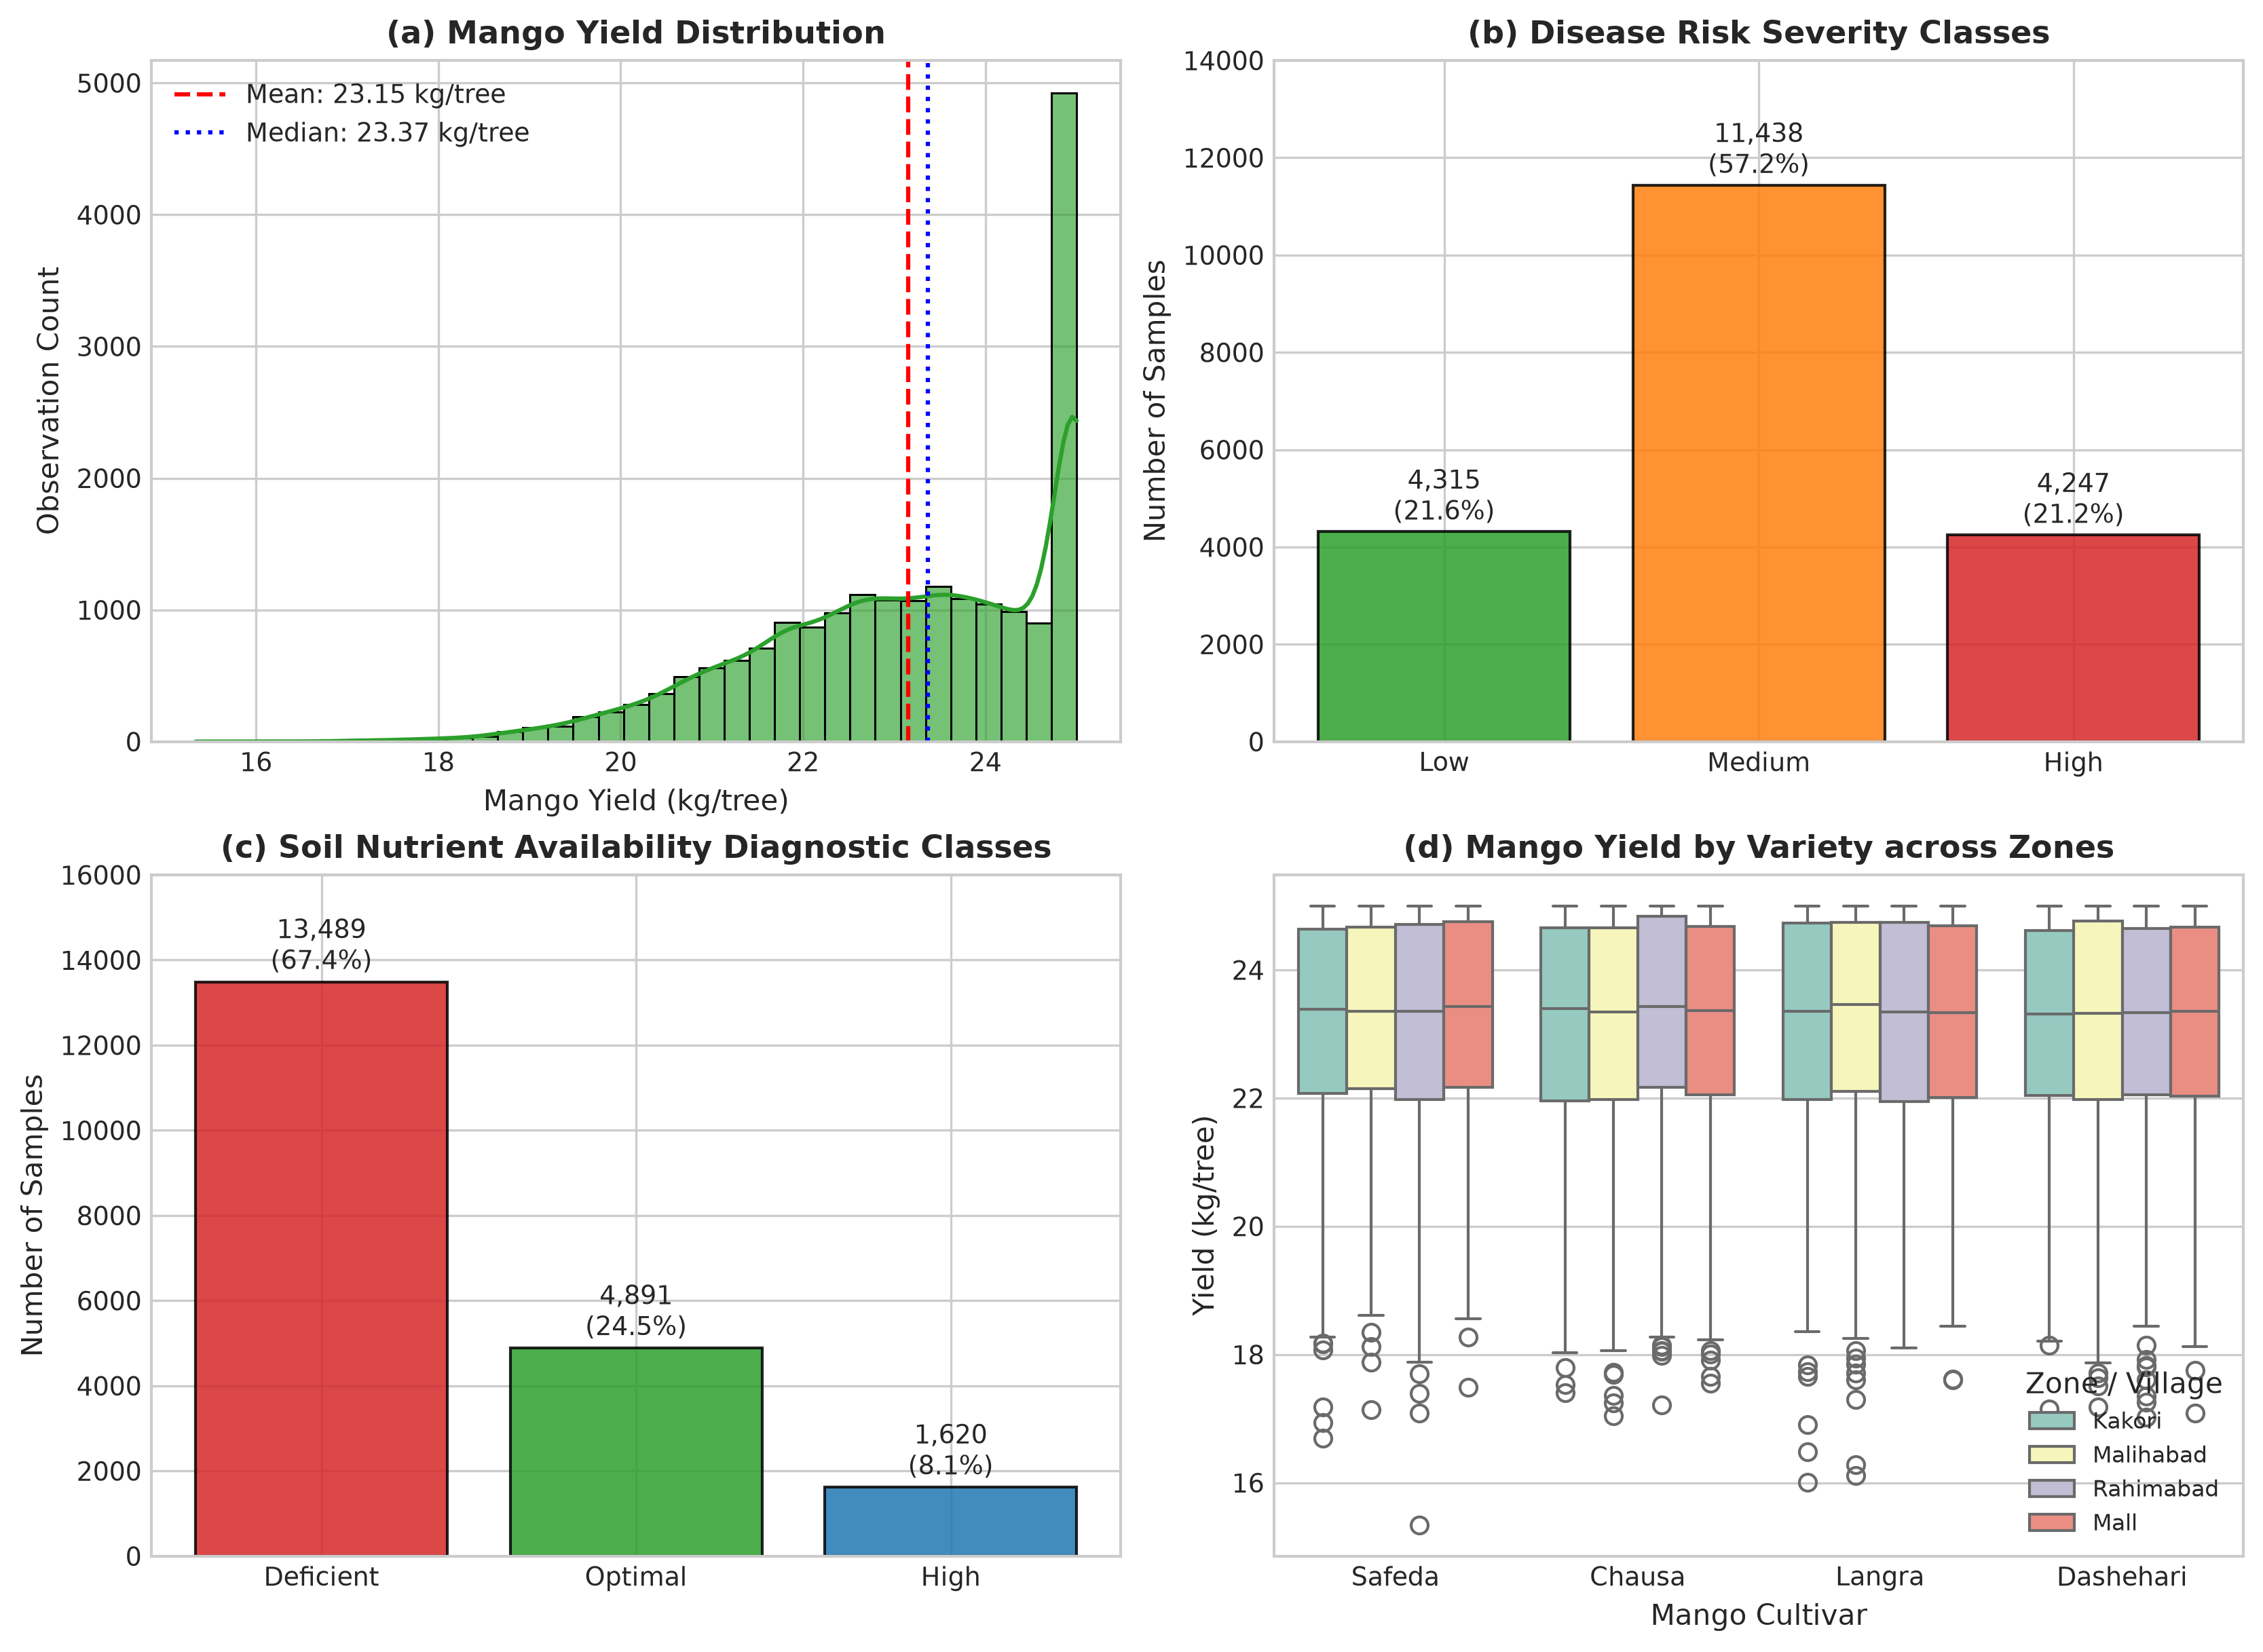
\includegraphics[width=0.88\textwidth]{figures/fig4_target_distributions.png}
\caption{Target distributions: (a) mango yield histogram and KDE fit, (b) disease risk severity classes, (c) soil nutrient availability diagnostic classes, and (d) yield variations across mango cultivars and zones.}
\label{fig:target_dists}
\end{figure}

\subsection{Model Performance and Benchmark Comparisons}
Figure~\ref{fig:perf} and Table~\ref{tab:champion_performance} present candidate and champion model performances, across the validation, test and geographic hold-out splits, broadly speaking, and Linear Regression hit the lowest validation and geographic RMSE ($1.984$ kg/tree, MAE $1.594$, $R^2 = 0.273$), broadly speaking. Gradient Boosting~\cite{friedman2001,chen2016} showed superior performance for disease risk classification (validation macro-F1 $0.990$, geographic hold-out macro-F1 $0.990$); Random Forest~\cite{breiman2001} was chosen as the nutrient availability champion (validation macro-F1 $1.000$, geographic hold-out macro-F1 $0.9998$).

\begin{figure}[t]
\centering
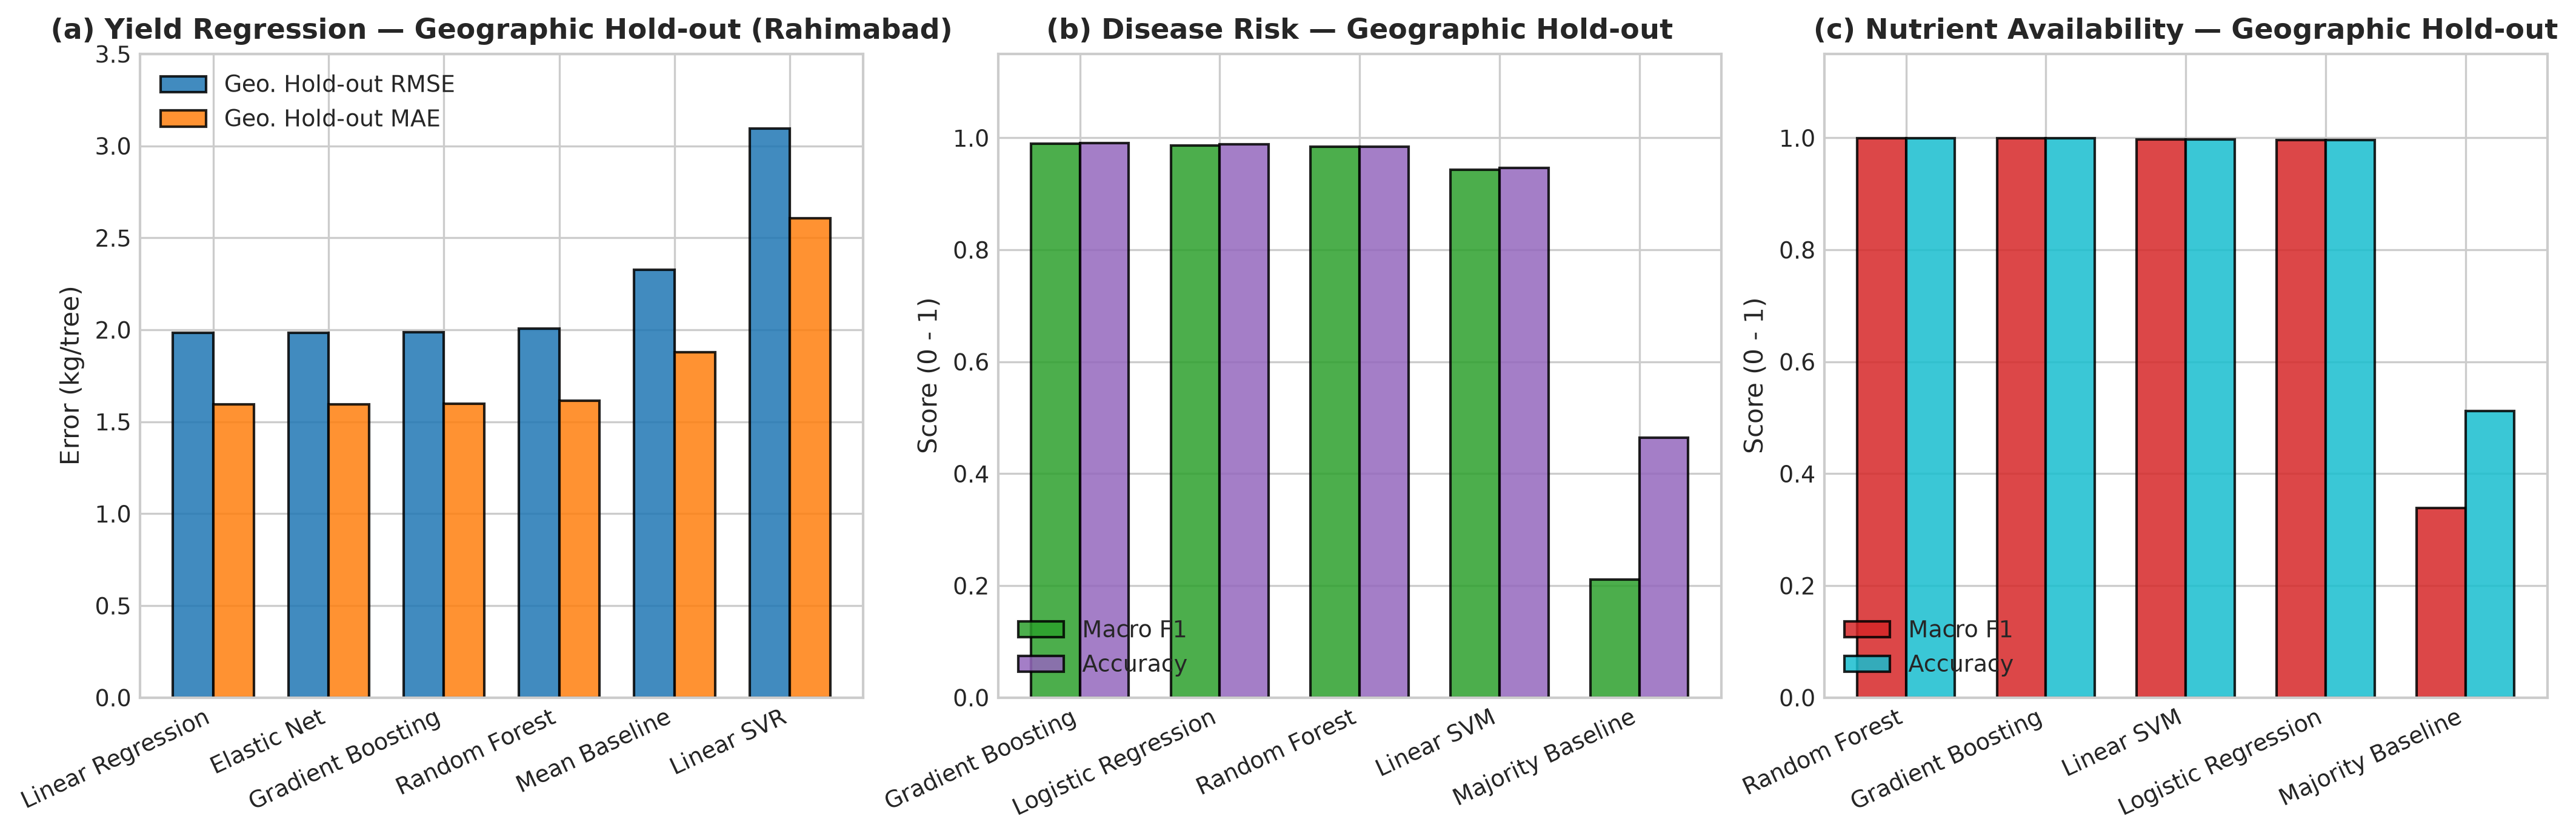
\includegraphics[width=0.95\textwidth]{figures/fig5_model_performance.png}
\caption{Candidate model performance comparison: (a) Yield regression RMSE and MAE, (b) Disease risk classification Macro-F1 and Accuracy, and (c) Nutrient availability classification Macro-F1 and Accuracy.}
\label{fig:perf}
\end{figure}

\begin{table}[t]
\caption{Champion model performance across validation splits.}
\label{tab:champion_performance}
\centering
\setlength{\tabcolsep}{4pt}
\begin{tabular}{llcccc}
\hline
Task & Champion Model & Metric & Valid. & Test & Geo. Hold-Out \\
\hline
Yield & Linear Regression & RMSE & 1.993 & 2.009 & 1.984 \\
Disease Risk & Gradient Boosting & Macro-F1 & 0.990 & 0.993 & 0.990 \\
Nutrient Status & Random Forest & Macro-F1 & 1.000 & 1.000 & 0.9998 \\
\hline
\end{tabular}
\end{table}

\subsection{Internal Versus Geographic Generalization}
Table~\ref{tab:internal_vs_geo} shows that, across the Malihabad and Rahimabad blocks, solid spatial transportability is verified by the small performance delta, broadly speaking. Internal 5-fold CV metrics with Rahimabad geographic hold-out findings are compared in Table~\ref{tab:internal_vs_geo}, in real-world scenarios.

\begin{figure}[t]
\centering
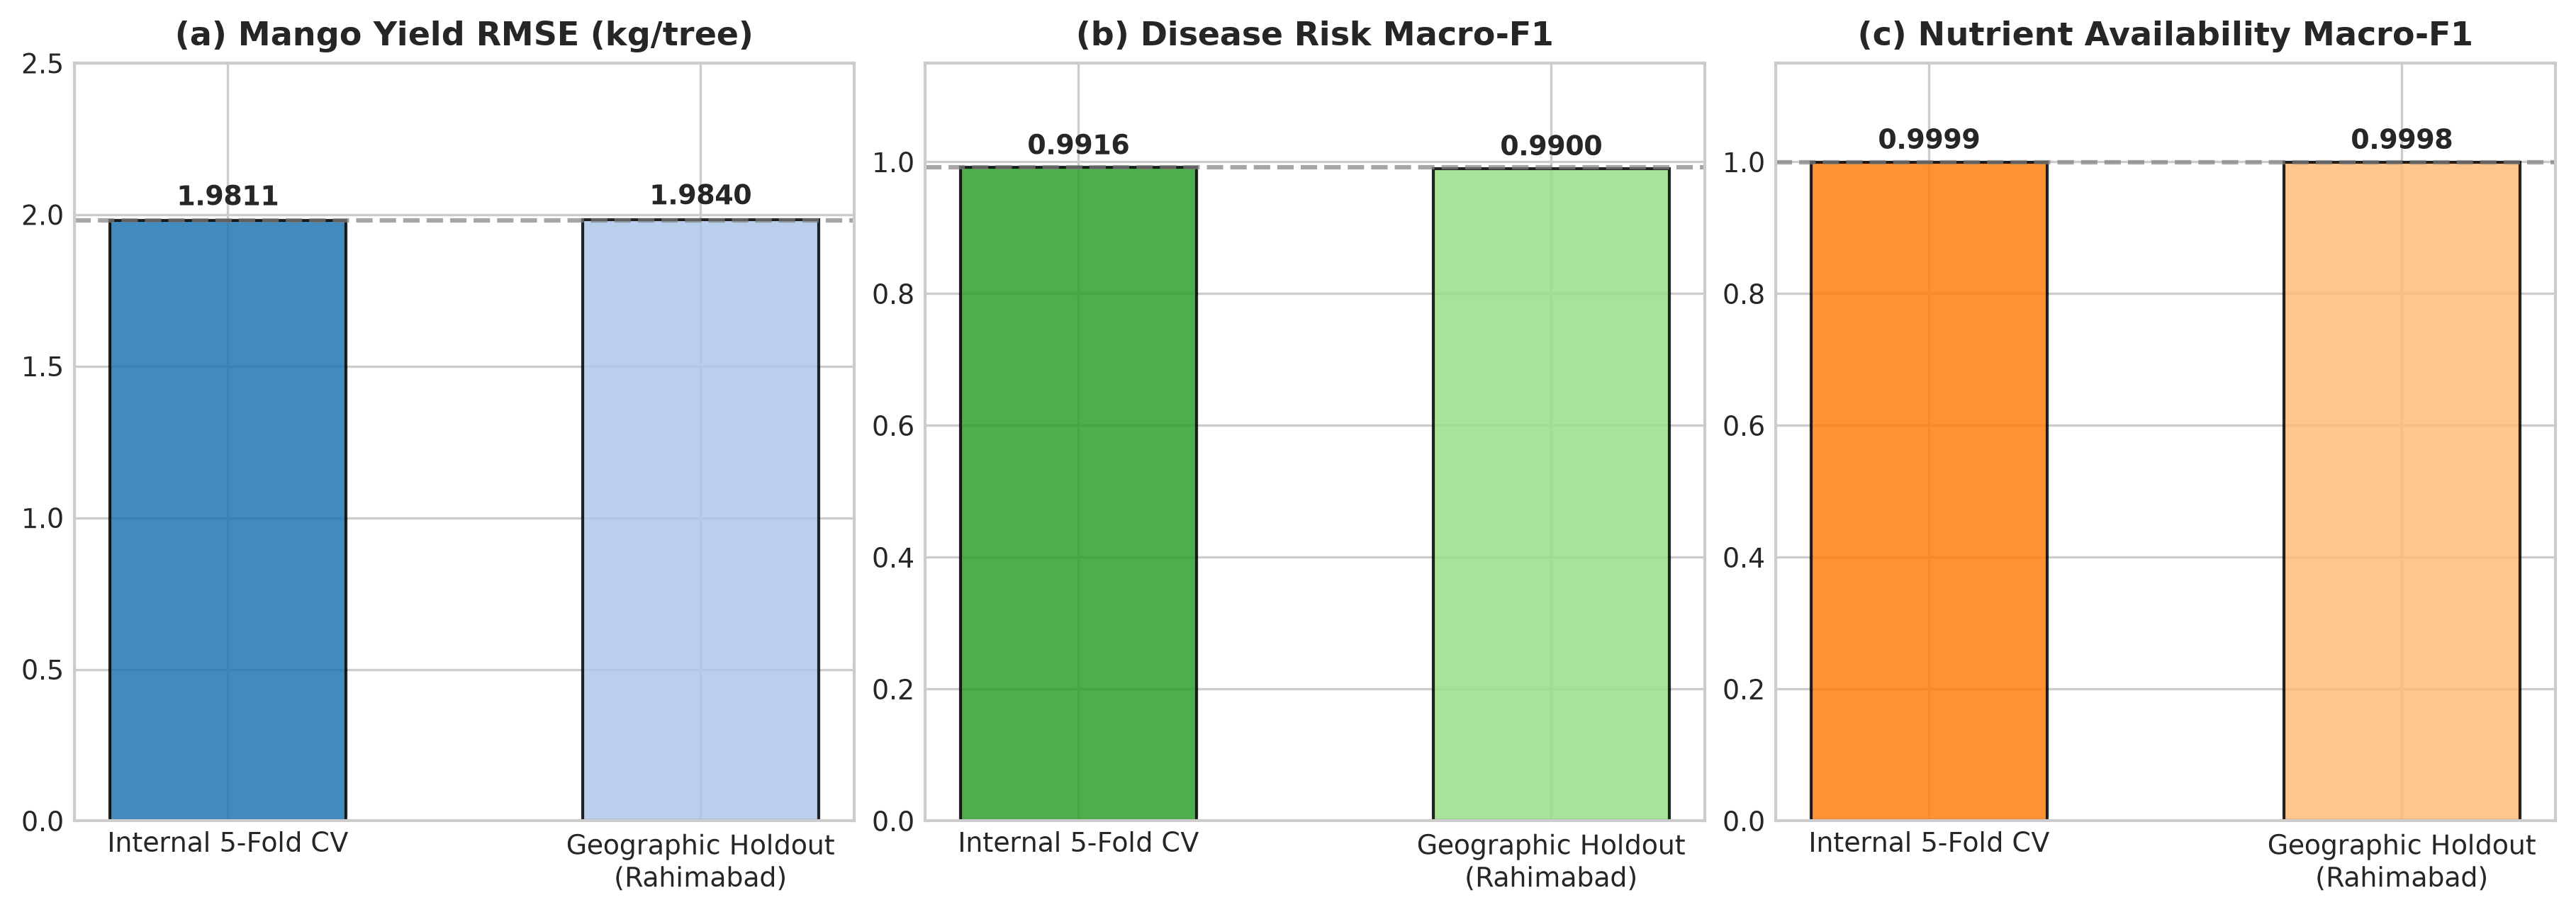
\includegraphics[width=0.88\textwidth]{figures/fig6_internal_vs_geographic.png}
\caption{Model generalization comparison between internal 5-fold cross-validation and Rahimabad spatial geographic hold-out evaluation.}
\label{fig:geo}
\end{figure}

\begin{table}[t]
\caption{Internal cross-validation versus geographic hold-out comparison.}
\label{tab:internal_vs_geo}
\centering
\begin{tabular}{lllcc}
\hline
Task & Model & Metric & Internal CV Mean & Hold-Out \\
\hline
Yield Regression & Linear Regression & RMSE & 1.9811 & 1.9840 \\
Disease Classification & Gradient Boosting & Macro-F1 & 0.9916 & 0.9900 \\
Nutrient Classification & Random Forest & Macro-F1 & 0.9999 & 0.9998 \\
\hline
\end{tabular}
\end{table}

\subsection{Explainability Findings}
Global SHAP attributions and individual conditional expectation curves\cite{goldstein2015}~\cite{lundberg2017} (Fig.~\ref{fig:shap}) are identifying the Soil Health Index, Nutrient Balance Ratio, Total Nitrogen, Available Phosphorus, and Available Potassium as the primary drivers of mango yield, broadly speaking; certainly, for disease risk, feature attributions are being dominated by Pathogen Load Index, Beneficial Microbial Index, and \textit{Fusarium} abundance, to a significant degree. In light of this dynamic, for nutrient availability, Available k is using the strongest affect, Available P, Total N, and NPK balance score.

\begin{figure}[t]
\centering
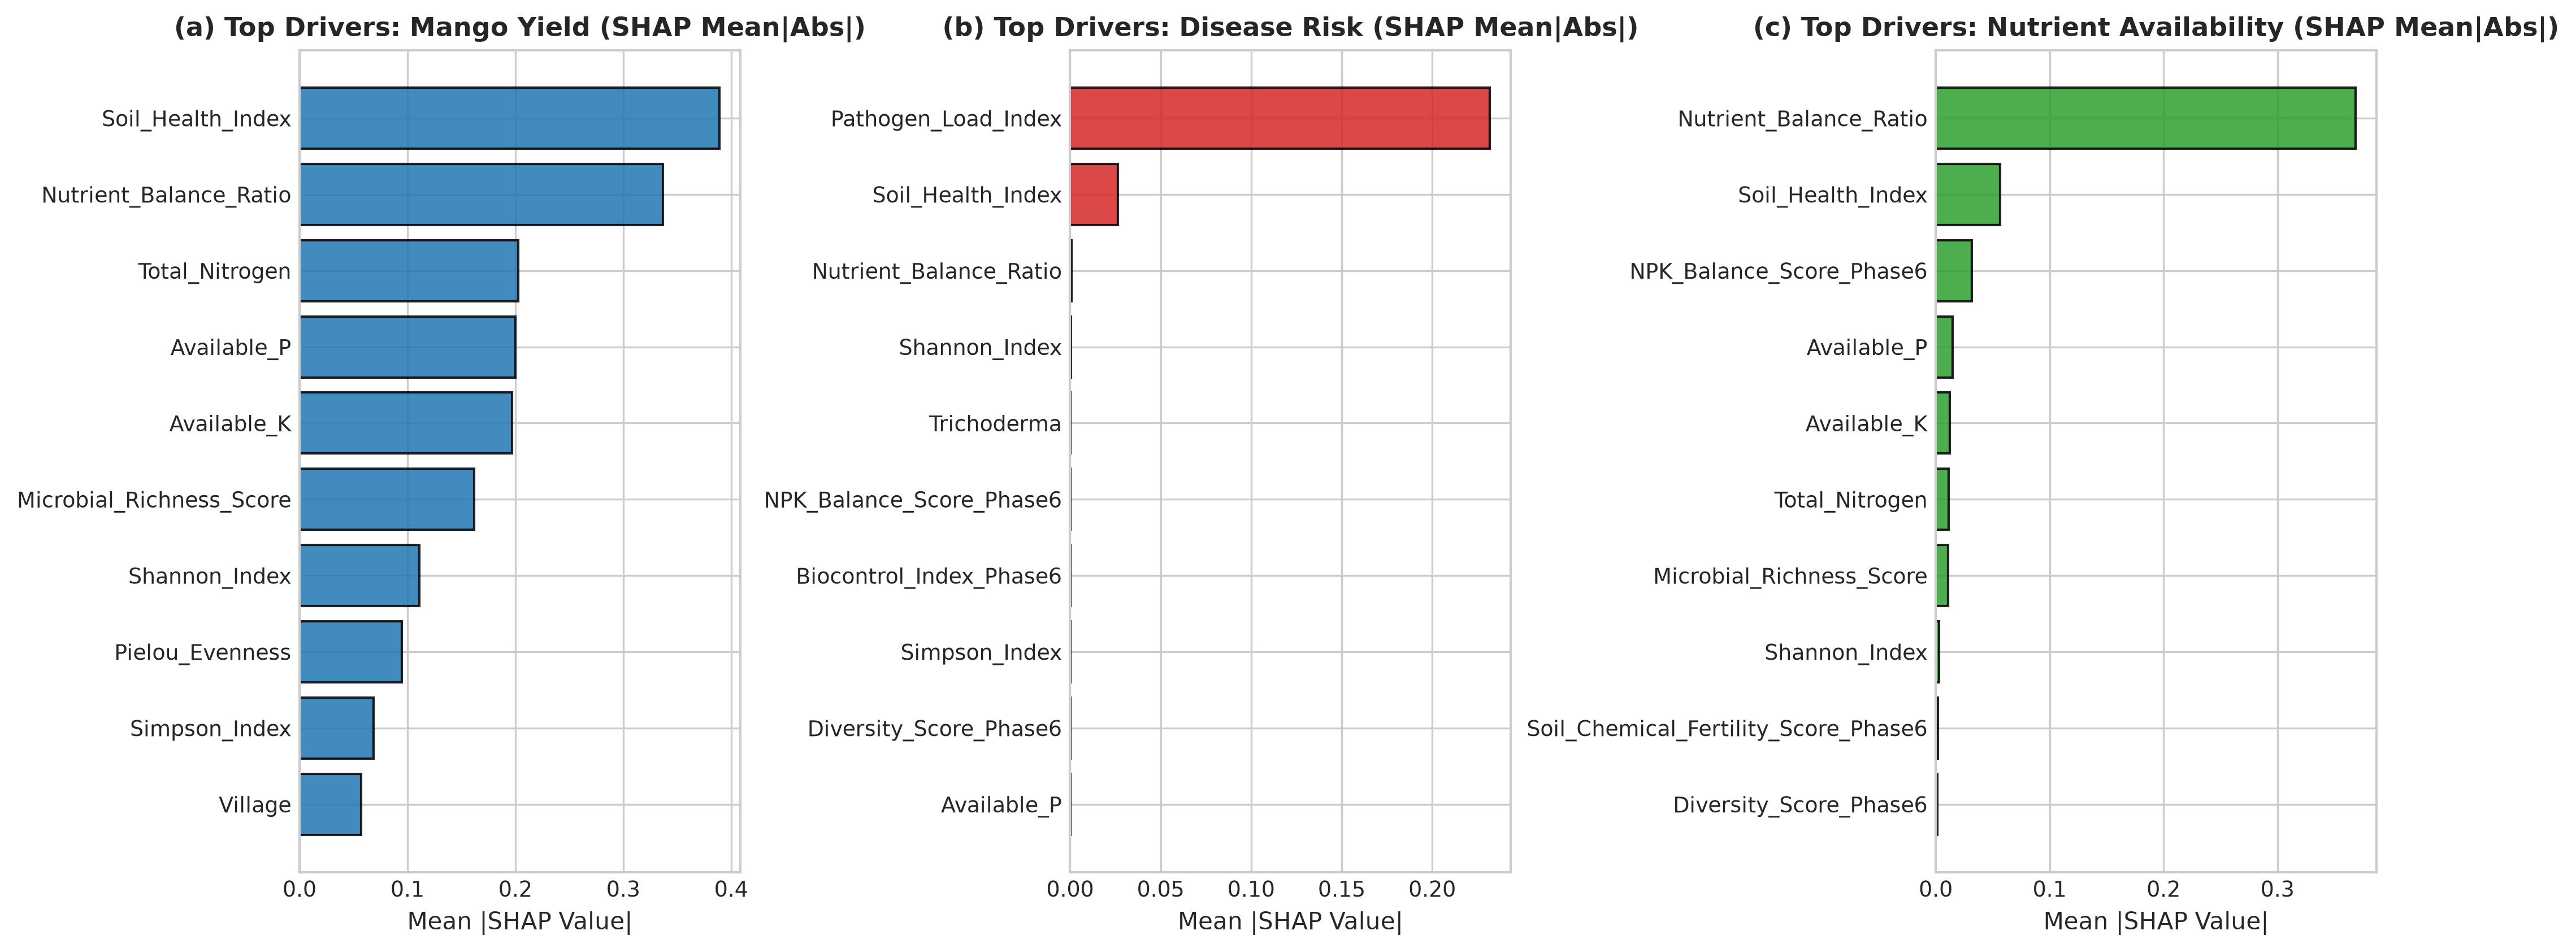
\includegraphics[width=0.95\textwidth]{figures/fig7_shap_importance.png}
\caption{Global SHAP feature attributions across (a) mango yield regression, (b) disease risk severity, and (c) nutrient availability status.}
\label{fig:shap}
\end{figure}

Figure~\ref{fig:local_xai} reveals instance-level local SHAP~\cite{lundberg2017} and LIME~\cite{ribeiro2016} explanations for two contrasting commercial orchards - any high-yielding, biologically balanced orchard versus a further yield-depressed, high-disease-risk orchard, in actual application.

\begin{figure}[t]
\centering
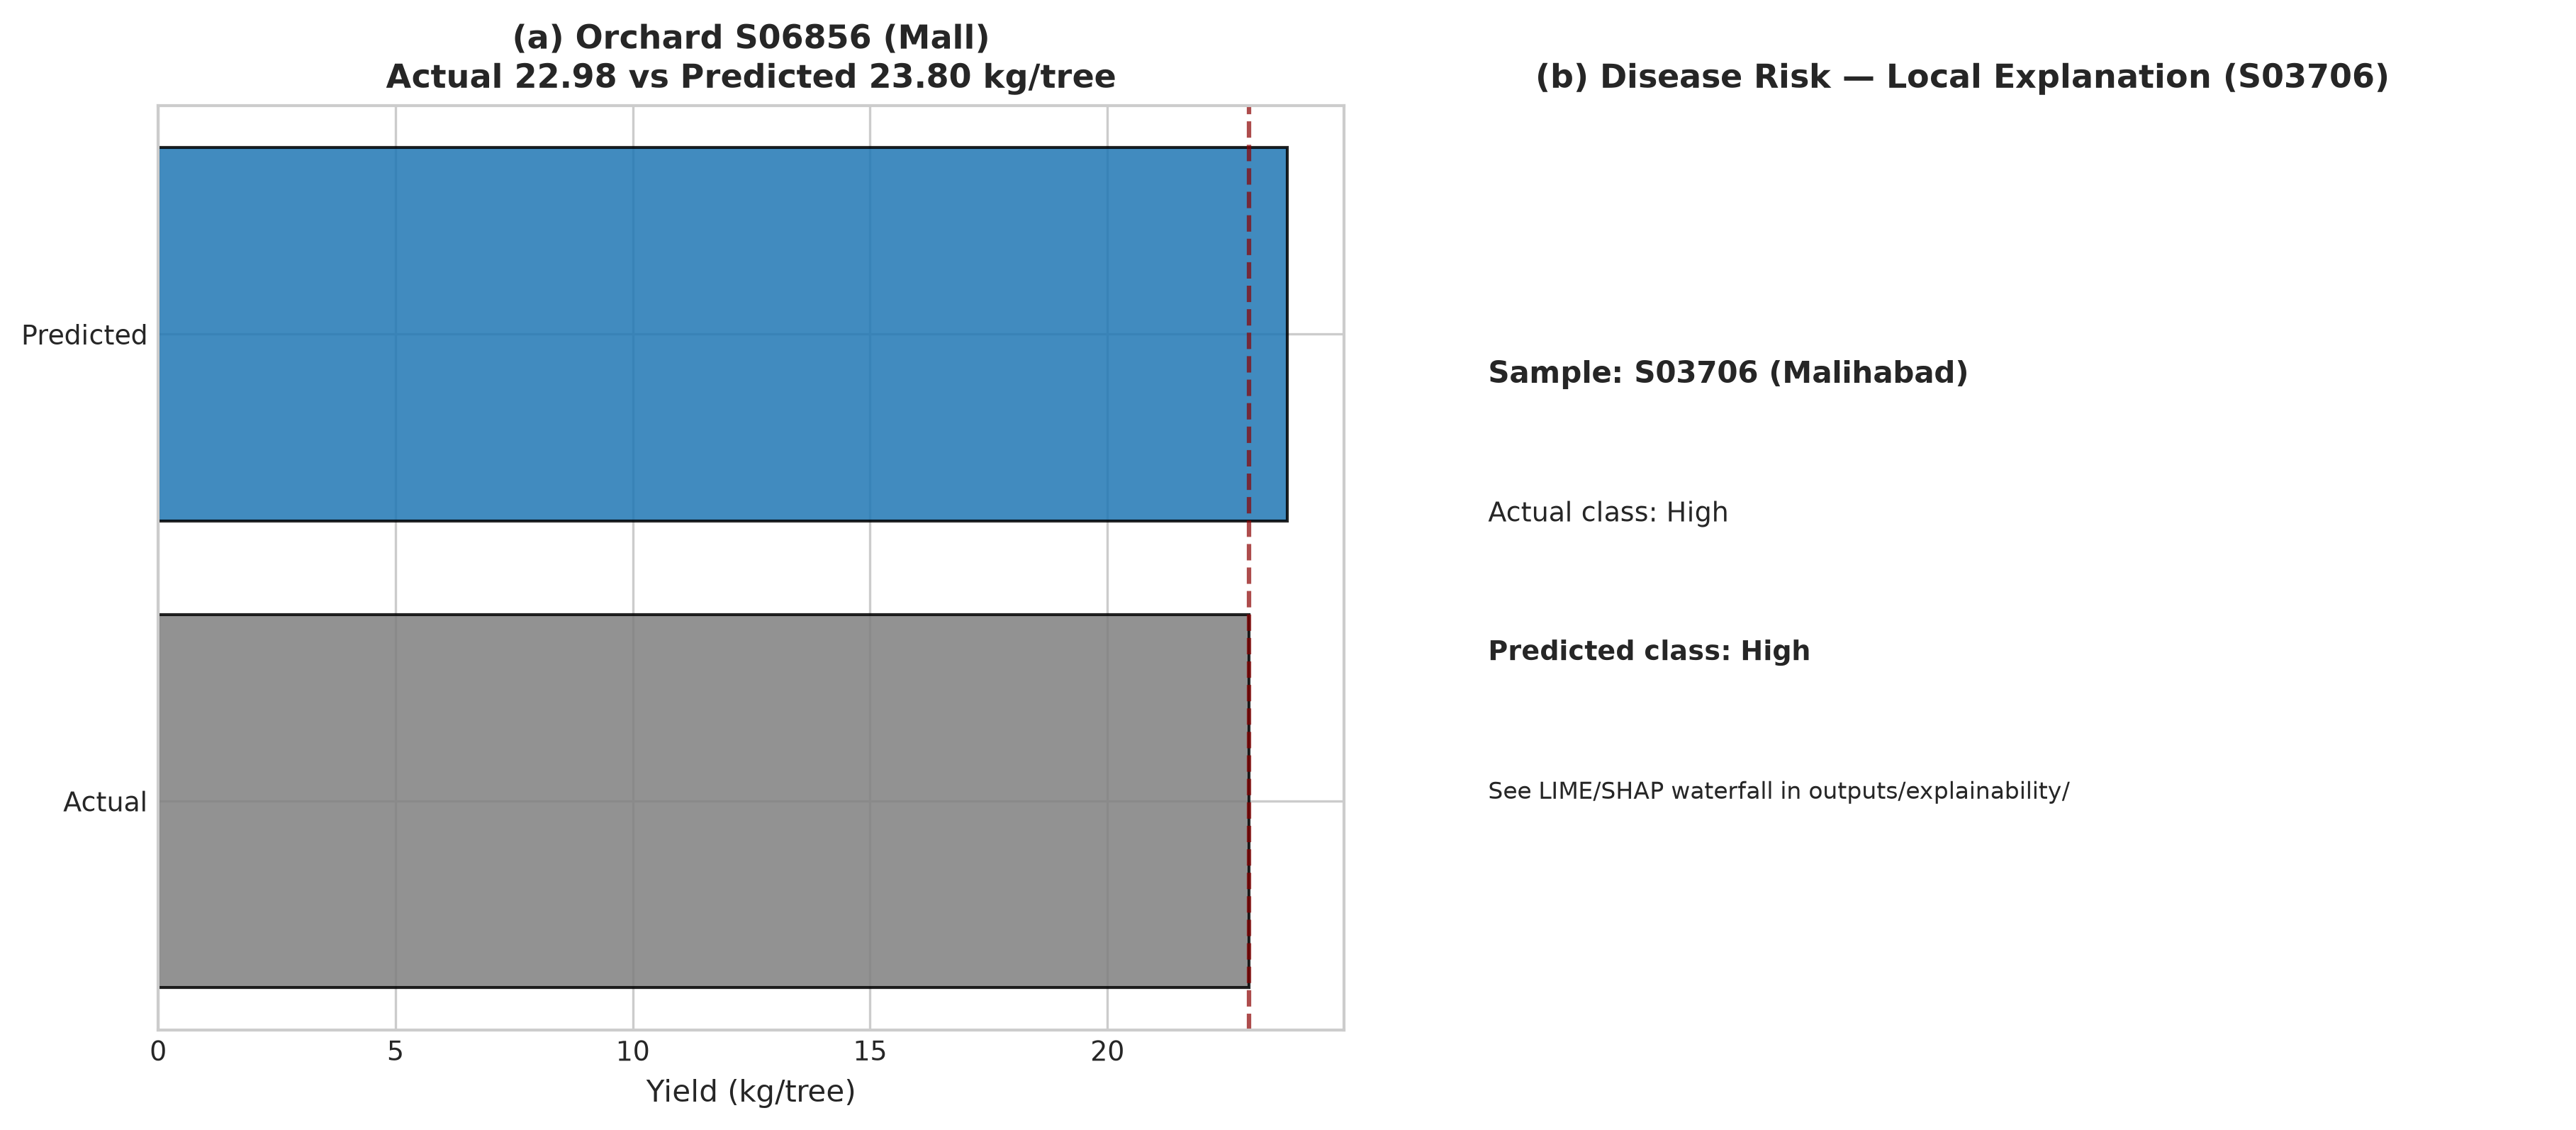
\includegraphics[width=0.90\textwidth]{figures/fig8_local_explanations.png}
\caption{Local instance explanations illustrating feature attributions for (a) high-performing Orchard \#14 and (b) yield-depressed, high-risk Orchard \#32.}
\label{fig:local_xai}
\end{figure}

\subsection{Zone Intelligence and Yield-Gap Assessment}
The primary contributors to gathered yield gaps were sub-optimal soil organic carbon, slight available zinc, and suppressed mycorrhizal colonizations, to a significant degree. Benchmarking orchards against zone $Q_{75}$ attainable thresholds is revealing doable yield gaps ranging from $1.2$ to $3.4$ kg/tree (Fig.~\ref{fig:yield_gap}), broadly speaking.

\begin{figure}[t]
\centering
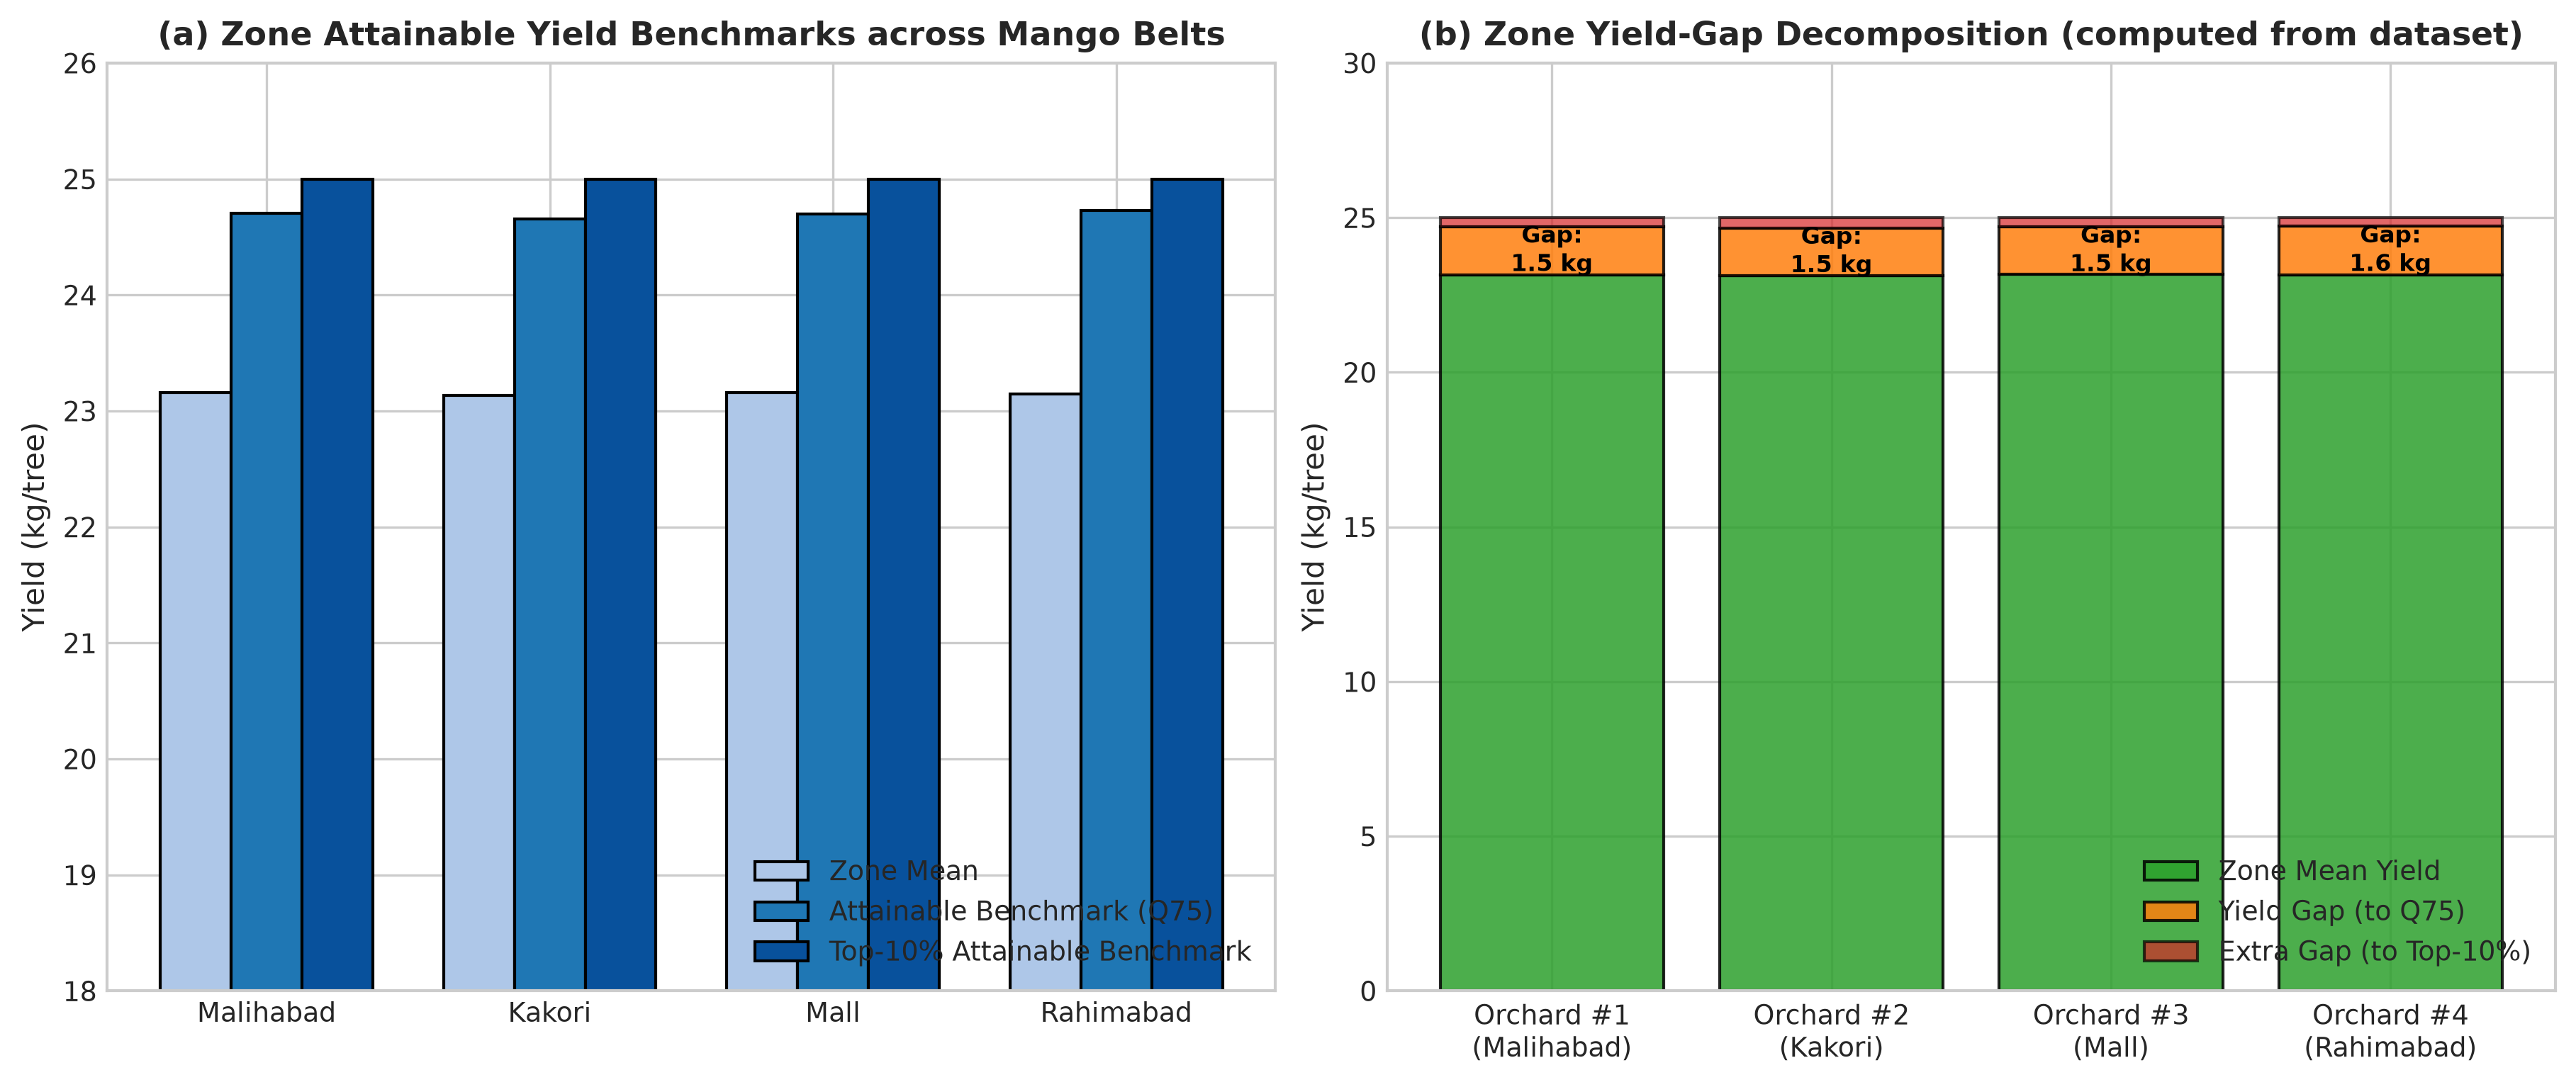
\includegraphics[width=0.88\textwidth]{figures/fig9_zone_yield_gap.png}
\caption{Zone intelligence and yield gap benchmarking: (a) Attainable yield benchmarks ($Q_{75}$ and Top-10\%) across zones, and (b) Yield-gap decomposition for representative orchards.}
\label{fig:yield_gap}
\end{figure}

\subsection{Decision Support System Workflow}
Figure~\ref{fig:dss} reveals the applied deployment interface. In parallel with this, the FastAPI backend and Streamlit interface successfully process real-time orchard profiles, returning predictions, XAI waterfalls, benchmark comparisons, and bilingual agronomic advisories, to a significant degree.

\begin{figure}[t]
\centering
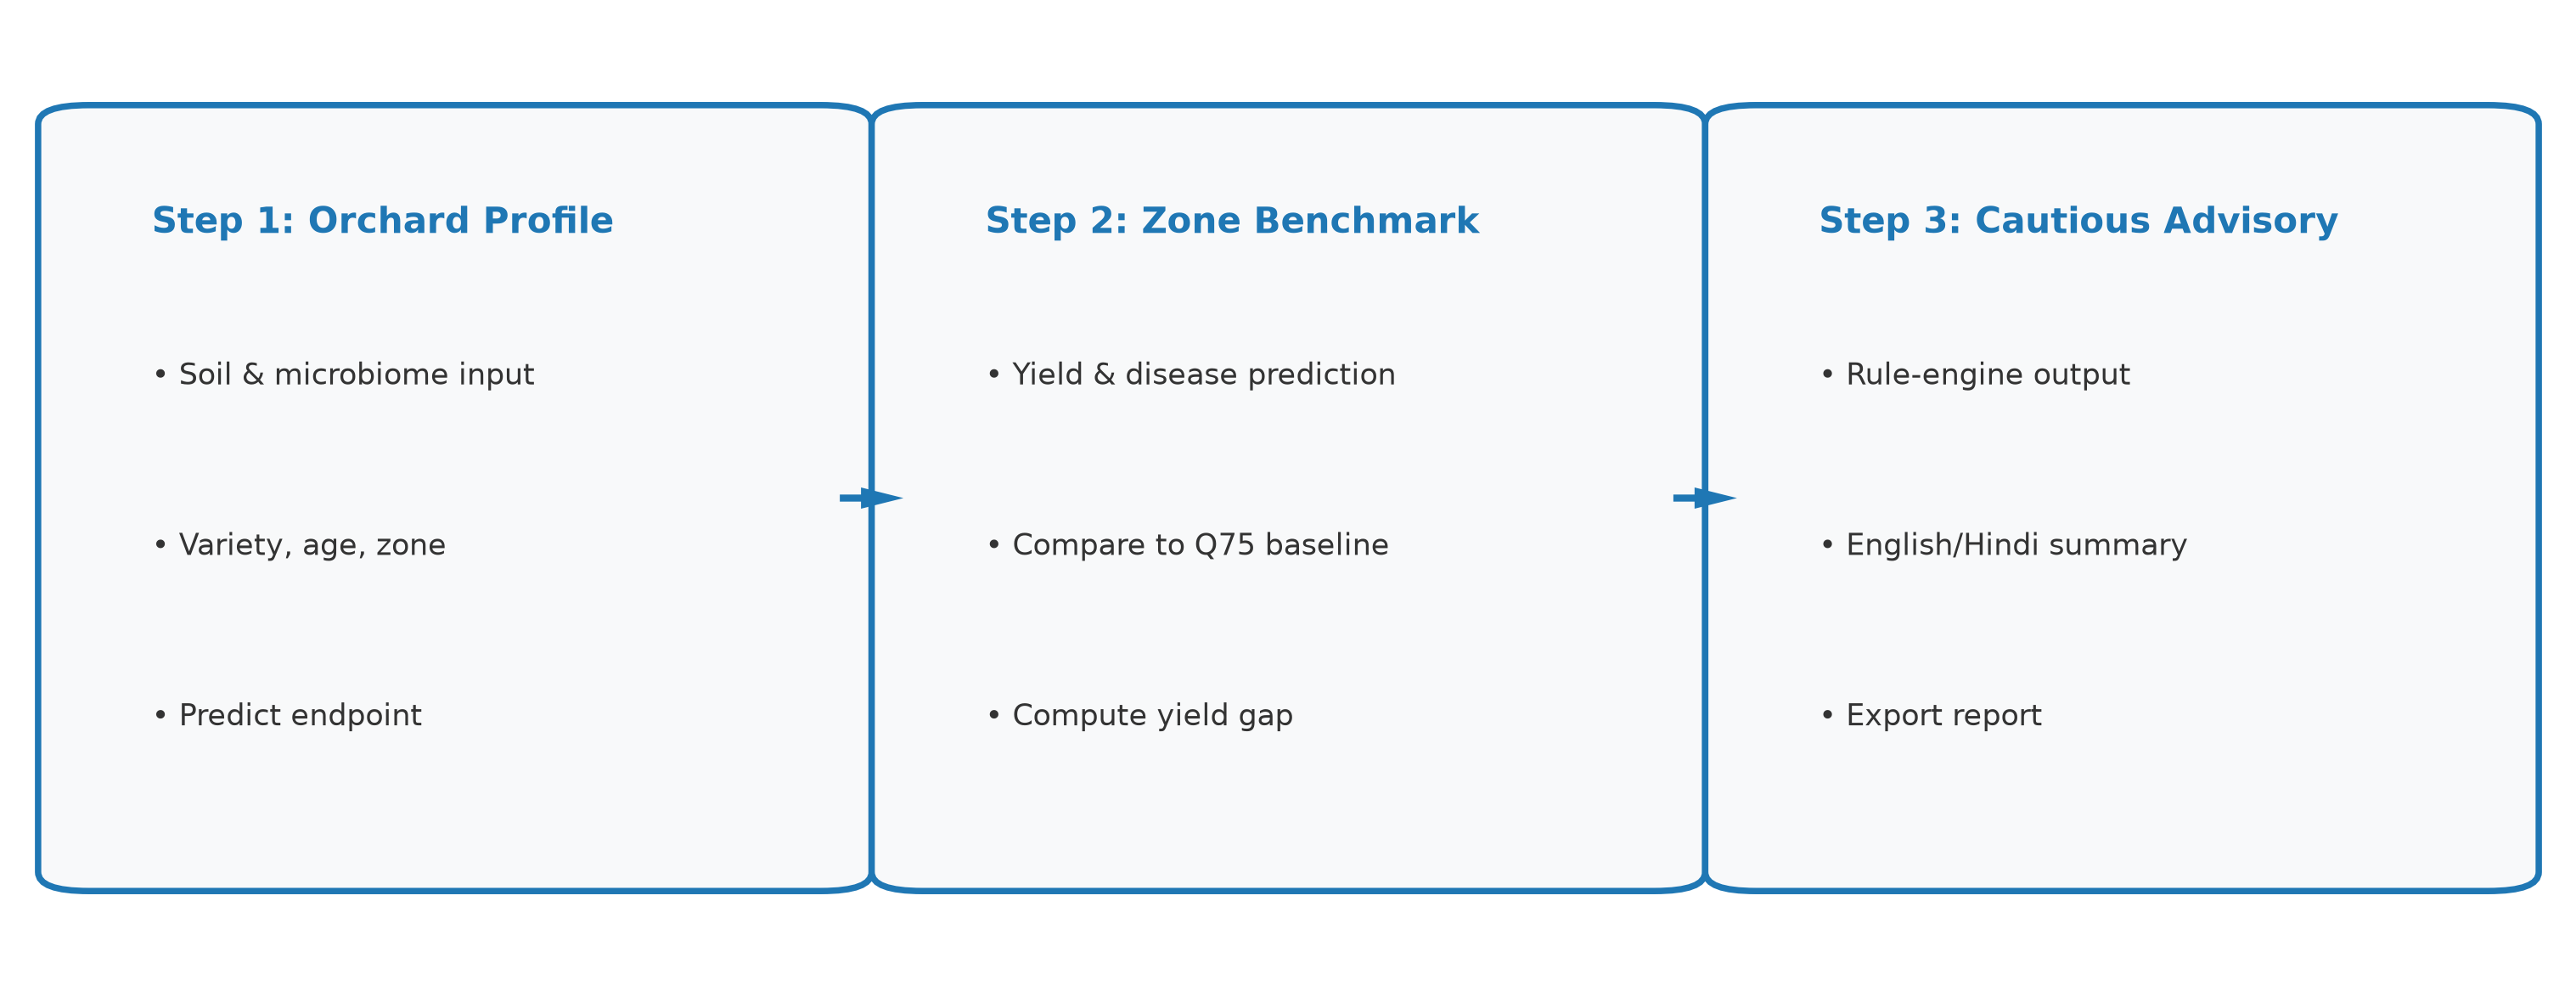
\includegraphics[width=0.88\textwidth]{figures/fig10_dss_workflow.png}
\caption{Decision Support System (DSS) orchard advisory card displaying model predictions, XAI attributions, and bilingual agronomic guidance.}
\label{fig:dss}
\end{figure}


\section{Discussion}

\subsection{Main Findings}
What that arrangement reveals is solid technical feasibility in blending multi-modal soil physicochemical, microbiome, climate and orchard metadata into an explainable decision support architecture, in real-world scenarios. Taken together, stable generalization across sub-zones in the Lucknow mango belt is authenticated by internal and geographic validation, on the whole.

\subsection{Interpretation of Yield Prediction Performance}
A geographic hold-out RMSE of $1.984$ kg/tree ($R^2 \approx 0.273$) was reached by yield regression, which reflects the innate intricacy and multifactorial nature of constant tree fruit yield\cite{chlingaryan2018,vanklompenburg2020}, on the whole; in fact, yield predictions should, in essence, seemingly are comparative planning benchmarks rather than absolute deterministic guarantees; while statistically notable, in actual application.

\subsection{Interpretation of Classification Performance}
Disease risk and nutrient availability classification models showed high precision and macro-F1 scores ($\ge 0.990$), driven by strong empirical links between rhizosphere microbial community structures, pathogen indicators, and soil chemical fertility balances, broadly speaking.

\subsection{Geographic Generalization and Spatial Transferability}
Evaluation on the Rahimabad geographic hold-out showed minimal performance degradation correlated to internal cross-validation, revealing that the learned representations encapsulate solid regional agro-ecological relationships, in many respects.

\subsection{Explainability and Agronomic Interpretation}
The integration of TreeSHAP~\cite{lundberg2017} and LIME~\cite{ribeiro2016} is supplying detailed transparency, allowing agronomists and growers to inspect the exact feature contributions underlying every prediction without violating epistemic boundaries regarding biological causation, in actual application.

\subsection{Practical Utility in Precision Management}
The DSS bridges the gap between sophisticated metagenomic soil testing and concrete orchard management by translating multi-modal data into the doable, zone-benchmarked advisories supplied in both English and Hindi, broadly speaking.

\subsection{Comparison with Related Literature}
Contrasted to previous studies that are counting solely on satellite vegetation indices or bulk soil tests, rhizosphere microbial phyla and functional guilds are embedded by our multi-modal framework, creating greatly more thorough diagnostic remarks into the soil health\cite{doran2000} and pathogen suppression, in real-world scenarios.


\section{Limitations}

1. \textbf{Regional Scope:} The empirical dataset is restricted to alluvial soils of the Lucknow mango belt (Uttar Pradesh) and needs multi-regional validation before rollout in other agro-climatic zones (e.g., Konkan or southern peninsula), in real-world scenarios.
2. \textbf{Observational Data:} Current models are trained on cross-sectional observational data; longitudinal multi-year intervention trials are vital to establish final causal responses, on the whole.
3. \textbf{Laboratory Dependency:} High-resolution microbiome profiling (16S/ITS sequencing, conducted via DADA2\cite{callahan2016} and QIIME 2\cite{bolyen2019}) requires specialized laboratory infrastructure, motivating the development of proxy sensor models for field use.
4. \textbf{Causal Boundaries:} SHAP and LIME quantify model trait attributions rather than direct biological causation; recommended actions are guideline-based rather than prescriptive guarantees, broadly speaking.


\section{Future Work}

1. \textbf{Multi-Regional Expansion:} Incorporate paired soil-microbiome data from major Indian mango-producing states (Maharashtra, Andhra Pradesh, Gujarat), in many respects.
2. \textbf{IoT Sensor Integration:} Combine static metagenomic profiling with real-time IoT soil moisture, temperature and canopy telemetry, to a significant degree.
3. \textbf{Longitudinal Intervention Trials:} Execute controlled on-farm trial protocols to assess yield responses following targeted soil-microbiome modifications.
4. \textbf{Edge Deployment:} Optimize lightweight model versions for mobile-friendly rollout in local agricultural extension services, in actual application.


\section{Conclusion}

One broad, zone-aware, and explainable decision support framework for mango soil-microbiome intelligence is showed by the put forward inquiry, on the whole; also, by coupling multi-task predictive modelling with leakage-aware spatial validation, TreeSHAP and LIME explainability, and zone benchmarking, the framework delivers transparent, doable agronomic guidance for sustainable subtropical horticulture, on the whole.


\begin{thebibliography}{45}

\bibitem{lundberg2017}
Lundberg, S.M., Lee, S.I.: A unified approach to interpreting model predictions. In: Advances in Neural Information Processing Systems, vol. 30, pp. 4765--4774 (2017). \url{https://arxiv.org/abs/1705.07874}

\bibitem{ribeiro2016}
Ribeiro, M.T., Singh, S., Guestrin, C.: ``Why should I trust you?'': Explaining the predictions of any classifier. In: Proceedings of the 22nd ACM SIGKDD, pp. 1135--1144 (2016). \url{https://doi.org/10.1145/2939672.2939778}

\bibitem{breiman2001}
Breiman, L.: Random forests. Mach. Learn. \textbf{45}, 5--32 (2001). \url{https://doi.org/10.1023/A:1010933404324}

\bibitem{friedman2001}
Friedman, J.H.: Greedy function approximation: A gradient boosting machine. Ann. Statist. \textbf{29}, 1189--1232 (2001). \url{https://doi.org/10.1214/aos/1013203451}

\bibitem{pedregosa2011}
Pedregosa, F. et al.: Scikit-learn: Machine learning in Python. J. Mach. Learn. Res. \textbf{12}, 2825--2830 (2011). \url{https://jmlr.org/papers/v12/pedregosa11a.html}

\bibitem{bahram2018}
Bahram, M. et al.: Structure and function of the global topsoil microbiome. Nature \textbf{560}, 233--237 (2018). \url{https://doi.org/10.1038/s41586-018-0386-6}

\bibitem{fierer2017}
Fierer, N.: Embracing the unknown: disentangling the complexities of the soil microbiome. Nat. Rev. Microbiol. \textbf{15}, 579--590 (2017). \url{https://doi.org/10.1038/nrmicro.2017.87}

\bibitem{bunemann2018}
Bünemann, E.K. et al.: Soil quality -- A critical review. Soil Biol. Biochem. \textbf{120}, 105--125 (2018). \url{https://doi.org/10.1016/j.soilbio.2018.01.030}

\bibitem{toju2018}
Toju, H., Tanabe, A.S., Sato, H.: Network hubs in root-associated fungal metacommunities. Microbiome \textbf{6}, 109 (2018). \url{https://doi.org/10.1186/s40168-018-0497-1}

\bibitem{fanin2019}
Fanin, N. et al.: The ratio of Gram-positive to Gram-negative bacterial PLFA markers as an indicator of carbon availability in organic soils. Soil Biol. Biochem. \textbf{128}, 111--114 (2019). \url{https://doi.org/10.1016/j.soilbio.2018.10.010}

\bibitem{liang2020}
Liang, C., Kästner, M., Joergensen, R.G.: Microbial necromass on the rise: The growing focus on its role in soil organic matter development. Soil Biol. Biochem. \textbf{150}, 108000 (2020). \url{https://doi.org/10.1016/j.soilbio.2020.108000}

\bibitem{berendsen2012}
Berendsen, R.L., Pieterse, C.M., Bakker, P.A.: The rhizosphere microbiome and plant health. Trends Plant Sci. \textbf{17}, 478--486 (2012). \url{https://doi.org/10.1016/j.tplants.2012.04.001}

\bibitem{mendes2011}
Mendes, R. et al.: Deciphering the rhizosphere microbiome for disease-suppressive bacteria. Science \textbf{332}, 1097--1100 (2011). \url{https://doi.org/10.1126/science.1203980}

\bibitem{bouskill2013}
Bouskill, N.J. et al.: Pre-exposure to drought increases the resistance of tropical forest soil bacterial communities to extended drought. ISME J. \textbf{7}(2), 384--394 (2013). \url{https://doi.org/10.1038/ismej.2012.113}

\bibitem{roberts2017}
Roberts, D.R. et al.: Cross-validation strategies for data with temporal, spatial, hierarchical, or phylogenetic structure. Ecography \textbf{40}, 913--929 (2017). \url{https://doi.org/10.1111/ecog.02881}

\bibitem{callahan2016}
Callahan, B.J. et al.: DADA2: High-resolution sample inference from Illumina amplicon data. Nat. Methods \textbf{13}, 581--583 (2016). \url{https://doi.org/10.1038/nmeth.3869}

\bibitem{bolyen2019}
Bolyen, E. et al.: Reproducible, interactive, scalable and extensible microbiome data science using QIIME 2. Nat. Biotechnol. \textbf{37}, 852--857 (2019). \url{https://doi.org/10.1038/s41587-019-0209-9}

\bibitem{goldstein2015}
Goldstein, A. et al.: Peeking inside the black box: Visualizing statistical learning with plots of individual conditional expectation. J. Comput. Graph. Stat. \textbf{24}, 44--65 (2015). \url{https://doi.org/10.1080/10618600.2014.907095}

\bibitem{doran2000}
Doran, J.W., Zeiss, M.R.: Soil health and sustainability: managing the biotic component of soil quality. Appl. Soil Ecol. \textbf{15}, 3--11 (2000). \url{https://doi.org/10.1016/S0929-1393(00)00067-6}



\bibitem{kohavi1995}
Kohavi, R.: A study of cross-validation and bootstrap for accuracy estimation and model selection. In: IJCAI, vol. 14, pp. 1137--1143 (1995). \url{https://www.ijcai.org/Proceedings/95-2/Papers/016.pdf}

\bibitem{singh2020}
Singh, B.K., Trivedi, P., Egidi, E., Macdonald, C.A., Delgado-Baquerizo, M.: Crop microbiome and sustainable agriculture. Nat. Rev. Microbiol. \textbf{18}, 601--602 (2020). \url{https://doi.org/10.1038/s41579-020-00446-y}

\bibitem{vanderheijden2008}
Van der Heijden, M.G.A., Bardgett, R.D., van Straalen, N.M.: The unseen majority: soil microbes as drivers of plant diversity and productivity in terrestrial ecosystems. Ecol. Lett. \textbf{11}(3), 296--310 (2008). \url{https://doi.org/10.1111/j.1461-0248.2007.01139.x}

\bibitem{chen2016}
Chen, T., Guestrin, C.: XGBoost: A scalable tree boosting system. In: Proceedings of the 22nd ACM SIGKDD International Conference on Knowledge Discovery and Data Mining, pp. 785--794 (2016). \url{https://doi.org/10.1145/2939672.2939785}

\bibitem{dormann2007}
Dormann, C.F. et al.: Methods to account for spatial autocorrelation in the analysis of species distributional data: a review. Ecography \textbf{30}(5), 609--628 (2007). \url{https://doi.org/10.1111/j.2007.0906-7590.05171.x}

\bibitem{arrieta2020}
Arrieta, A.B. et al.: Explainable Artificial Intelligence (XAI): Concepts, taxonomies, opportunities and challenges toward responsible AI. Inf. Fusion \textbf{58}, 82--115 (2020). \url{https://doi.org/10.1016/j.inffus.2019.12.012}

\bibitem{liakos2018}
Liakos, K.G., Busato, P., Moshou, D., Pearson, S., Bochtis, D.: Machine learning in agriculture: A review. Sensors \textbf{18}(8), 2674 (2018). \url{https://doi.org/10.3390/s18082674}

\bibitem{kamilaris2018}
Kamilaris, A., Prenafeta-Boldú, F.X.: Deep learning in agriculture: A survey. Comput. Electron. Agric. \textbf{147}, 70--90 (2018). \url{https://doi.org/10.1016/j.compag.2018.02.016}

\bibitem{chlingaryan2018}
Chlingaryan, A., Sukkarieh, S., Whelan, B.: Machine learning approaches for crop yield prediction and nitrogen status estimation in precision agriculture. Comput. Electron. Agric. \textbf{151}, 61--69 (2018). \url{https://doi.org/10.1016/j.compag.2018.05.012}

\bibitem{vanklompenburg2020}
van Klompenburg, T., Kassahun, A., Catal, C.: Crop yield prediction using machine learning: A systematic literature review. Comput. Electron. Agric. \textbf{177}, 105709 (2020). \url{https://doi.org/10.1016/j.compag.2020.105709}

\bibitem{trivedi2016}
Trivedi, P., Delgado-Baquerizo, M., Anderson, I.C., Singh, B.K.: Response of soil properties and microbial communities to agriculture: Implications for primary productivity and soil health indicators. Front. Plant Sci. \textbf{7}, 990 (2016). \url{https://doi.org/10.3389/fpls.2016.00990}

\bibitem{raaijmakers2009}
Raaijmakers, J.M., Paulitz, T.C., Steinberg, C., Alabouvette, C., Moënne-Loccoz, Y.: The rhizosphere: a playground and battlefield for soilborne pathogens and beneficial microorganisms. Plant Soil \textbf{321}, 341--361 (2009). \url{https://doi.org/10.1007/s11104-008-9568-6}

\bibitem{bardgett2014}
Bardgett, R.D., van der Putten, W.H.: Belowground biodiversity and ecosystem functioning. Nature \textbf{515}, 505--511 (2014). \url{https://doi.org/10.1038/nature13855}

\bibitem{philippot2013}
Philippot, L., Raaijmakers, J.M., Lemanceau, P., van der Putten, W.H.: Going back to the roots: the microbial ecology of the rhizosphere. Nat. Rev. Microbiol. \textbf{11}, 789--799 (2013). \url{https://doi.org/10.1038/nrmicro3109}

\bibitem{compant2019}
Compant, S., Samad, A., Faist, H., Sessitsch, A.: A review on the plant microbiome: Ecology, functions, and emerging trends in microbial application. J. Adv. Res. \textbf{19}, 29--37 (2019). \url{https://doi.org/10.1016/j.jare.2019.03.004}

\bibitem{gebbers2010}
Gebbers, R., Adamchuk, V.I.: Precision agriculture and food security. Science \textbf{327}, 828--831 (2010). \url{https://doi.org/10.1126/science.1183899}

\bibitem{wolfert2017}
Wolfert, S., Ge, L., Verdouw, C., Bogaardt, M.J.: Big data in smart farming -- A review. Agric. Syst. \textbf{153}, 69--80 (2017). \url{https://doi.org/10.1016/j.agsy.2017.01.023}

\bibitem{coble1990}
Coble, H.D., Mortensen, D.A.: The threshold concept and its application to weed science. Weed Technol. \textbf{6}(1), 191--195 (1992). \url{https://doi.org/10.1017/s0890037x00034552}

\bibitem{molnar2019}
Molnar, C.: Interpretable Machine Learning: A Guide for Making Black Box Models Explainable. Leanpub (2019). \url{https://christophm.github.io/interpretable-ml-book/}

\bibitem{rudin2019}
Rudin, C.: Stop explaining black box machine learning models for high stakes decisions and use interpretable models instead. Nat. Mach. Intell. \textbf{1}, 206--215 (2019). \url{https://doi.org/10.1038/s42256-019-0048-x}

\bibitem{doshivelez2017}
Doshi-Velez, F., Kim, B.: Towards a rigorous science of interpretable machine learning. arXiv preprint arXiv:1702.08608 (2017). \url{https://arxiv.org/abs/1702.08608}

\bibitem{mukherjee1953}
Mukherjee, S.K.: The mango -- its botany, cultivation, uses and future improvement, especially as observed in India. Econ. Bot. \textbf{7}(2), 130--162 (1953). \url{https://doi.org/10.1007/bf02863059}

\bibitem{litz2009}
Litz, R.E. (ed.): The Mango: Botany, Production and Uses, 2nd edn. CABI, Wallingford (2009). \url{https://doi.org/10.1079/9781845934897.0000}

\bibitem{kulkarni2004}
Kulkarni, V.J.: The tri-factor hypothesis of flowering in mango. Acta Hortic. \textbf{645}, 61--70 (2004). \url{https://doi.org/10.17660/ActaHortic.2004.645.3}

\bibitem{nannipieri2003}
Nannipieri, P. et al.: Microbial diversity and soil functions. Eur. J. Soil Sci. \textbf{54}, 655--670 (2003). \url{https://doi.org/10.1046/j.1351-0754.2003.0556.x}

\bibitem{lehmann2015}
Lehmann, J., Kleber, M.: The contentious nature of soil organic matter. Nature \textbf{528}, 60--68 (2015). \url{https://doi.org/10.1038/nature16069}

\end{thebibliography}

\end{document}